\documentclass[degree=master,language=english]{thuthesis}
% 选项
%   degree=[bachelor|master|doctor|postdoctor], % 必选,学位类型
%   language=[chinese|english], % 可选(默认:chinese),论文的主要语言
%   secret,                % 可选(默认:关闭),是否有密级
%   tocarialchapter,       % 可选(默认:关闭),章目录中使用黑体(这项表示同时打开下面两项)
%   tocarialchapterentry,  % 可选(默认:关闭),单独控制章标题在目录中使用黑体
%   tocarialchapterpage,   % 可选(默认:关闭),单独控制章页码在目录中使用黑体

% 所有其它可能用到的包都统一放到这里了,可以根据自己的实际添加或者删除。
\usepackage{thuthesis}
\usepackage{makecell}

% 定义所有的图片文件在 figures 子目录下
\graphicspath{{figures/}}

% 可以在这里修改配置文件中的定义。导言区可以使用中文。
% \def\myname{薛瑞尼}

% \renewcommand\bibname{References}
\begin{document}


%%% 封面部分
\frontmatter
\thusetup{
  %******************************
  % 注意:
  %   1. 配置里面不要出现空行
  %   2. 不需要的配置信息可以删除
  %******************************
  %
  %=====
  % 秘级
  %=====
  secretlevel={秘密},
  secretyear={10},
  %
  %=========
  % 中文信息
  %=========
  ctitle={基于触摸屏与柔性导电材料的大规模触摸交互技术研究},
  cdegree={工学硕士},
  cdepartment={全球创新学院},
  cmajor={数据科学与信息技术},
  cauthor={周建宇},
  csupervisor={喻\hspace{1.1cm} 纯 副研究员},
  cassosupervisor={王运涛 助理研究员}, % 副指导老师
%   ccosupervisor={某某某教授}, % 联合指导老师
  % 日期自动使用当前时间,若需指定按如下方式修改:
  cdate={二〇一九年十二月},
  %
  % 博士后专有部分
%   catalognumber     = {分类号},  % 可以留空
%   udc               = {UDC},  % 可以留空
%   id                = {编号},  % 可以留空: id={},
%   cfirstdiscipline  = {计算机科学与技术},  % 流动站(一级学科)名称
%   cseconddiscipline = {系统结构},  % 专 业(二级学科)名称
%   postdoctordate    = {2009 年 7 月——2011 年 7 月},  % 工作完成日期
%   postdocstartdate  = {2009 年 7 月 1 日},  % 研究工作起始时间
%   postdocenddate    = {2011 年 7 月 1 日},  % 研究工作期满时间
  %
  %=========
  % 英文信息
  %=========
  etitle={FlexTouch: Enabling Large-Scale Interaction Sensing beyond Touchscreens using Flexible and Conductive Materials},
  % 这块比较复杂,需要分情况讨论:
  % 1. 学术型硕士
  %    edegree:必须为Master of Arts或Master of Science(注意大小写)
  %             “哲学、文学、历史学、法学、教育学、艺术学门类,公共管理学科
  %              填写Master of Arts,其它填写Master of Science”
  %    emajor:“获得一级学科授权的学科填写一级学科名称,其它填写二级学科名称”
  % 2. 专业型硕士
  %    edegree:“填写专业学位英文名称全称”
  %    emajor:“工程硕士填写工程领域,其它专业学位不填写此项”
  % 3. 学术型博士
  %    edegree:Doctor of Philosophy(注意大小写)
  %    emajor:“获得一级学科授权的学科填写一级学科名称,其它填写二级学科名称”
  % 4. 专业型博士
  %    edegree:“填写专业学位英文名称全称”
  %    emajor:不填写此项
  edegree={Master of Science },
  emajor={Data Science and Information Technology},
  eauthor={Jianyu Zhou},
  esupervisor={Associate Professor Yu Chun},
  eassosupervisor={Assistant Professor Wang Yuntao},
  % 日期自动生成,若需指定按如下方式修改:
  edate={December, 2019},
  %
  % 关键词用“英文逗号”分割
  ckeywords={电容感应, 交互接口, 低成本制造, 2D电路设计, 大规模交互},
  ekeywords={Capacitive Sensing, Touch Interface, Low-cost Fabrication, 2D Circuit Pattern, Large-Scale Interaction},
}

% 定义中英文摘要和关键字
\begin{cabstract}
  目前基于感应电容的触摸屏交互已得到大规模应用,极大改变了人机交互模式,使人机交互更自然更、高效。然而,手机、平板电脑等电容屏设备的交互面积仍十分有限,很多情况下无法满足人们对更大规模的触摸交互需求,如桌面交互。而如果电容屏过大,第一不方便携带,第二制造成本也会大幅上升。如何在不改变现有触摸屏设备的基础上增加交互面积,成为了当前人机交互领域的一个热点研究方向,而本文的工作则是研究如何利用基于以手机为代表的智能交互设备的计算能力和电容特性,以低成本的方式将人机交互的平面从屏幕表面解放出来,扩展至计算设备周围更大的平面,满足用户大规模交互需求。

  本文提出了一种新的技术,使用廉价易得的导电材料即可在不改变交互设备本身的前提下大大增加交互面积,我们称为FlexTouch。我们利用柔性导电材料如铜铂线,将触摸屏的边缘与交互平面通过定制化的2D纸电路相连接,从而实现大规模交互,这种交互技术无需对已有设备做任何改造。我们通过实验证明了FlexTouch可应用于多种导电材料,包括铜箔胶带(copper foil tape)、纳米银墨(silver nanoparticle ink)、氧化铟锡薄膜(ITO film)和碳涂料(carbon paint),同时也适用于多种制造工艺,包括剪切技术、表面涂层技术和油墨喷印技术。我们的一系列研究和实验表明,FlexTouch可识别4米以内的人体触摸和2米以内的物体感知。最后,基于我们的识别原理和实验结果,我们展示了FlexTouc在不同场景下应用的可行性,例如可以在瑜伽垫上识别人体姿势,在桌面上检测人与水杯等物体的状态,以及在跑步机上检测人体的运动情况等。 Flextouch相比于之前的技术主要有以下优势:1)交互设备无需外部供电,可直接利用手机等智能设备的电源;2)改造简单,几乎无需改造交互平面,只需通过设计好的交互接口使手机/平板电脑与交互平面连接即可;3)改造成本低,实验所使用的柔性导电材料廉价易得。4)同时支持一维和二维交互,增加了有限面积内的感应密度。
    
  本文重点研究了1)不同导电材料对电容信号的影响,给出了不同材料的交互面积上限,为应用设计给出了理论指导;2)引入接地线后对电容感应信号的影响,进一步增强了信号识别率,为大范围交互提供了可能;3)多种不同的大范围纸电路设计和相应的交互应用场景,为更多不同模态的交互模式提供了参考;4)各种示例应用的在鲁棒性、准确性等方面的实际测试表现,证明了技术的可行性。
    
\end{cabstract}

% 如果习惯关键字跟在摘要文字后面,可以用直接命令来设置,如下:
% \ckeywords{\TeX, \LaTeX, CJK, 模板, 论文}

\begin{eabstract}
  Capacitive Touchscreens has been widely adopted in rencent ten years, greatly improved the effectiveness of human-computer interaction, enabling more natrual, more efficient interaction patterns. However, the interaction area of smartphone and tablet is still limited to the area of screen surface, which in many cases cannot meet the demands of large-scale interaction, such as table-based interaction. A straitforward solution to this issue is naively increase the area of touchscreen. However, there are at least two drawbacks: 1) Portability, 2) Cost Effectiveness. How to fully leverage existing smart device to enalbie large-scale interaction without modifications of smart device itself has become a popular research topic in Human-Computer Interaction.

  In this paper, we present FlexTouch, a technique that enables large-scale interaction sensing beyond the spatial constraints of capacitive touchscreens using passive low-cost conductive materials. This is achieved by customizing 2D circuit-like patterns with an array of conductive strips that can be easily attached to the sensing nodes on the edge of the touchscreen. This retrofit requires no hardware modification to the device. FlexTouch is compatible with various conductive materials (copper foil tape, silver nanoparticle ink, ITO frame, and carbon paint), as well as fabrication methods (cutting, coating, and ink-jet printing). We demonstrate that FlexTouch can support long-range touch sensing for up to 4 meters and everyday object presence detection for up to 2 meters. Finally, we show the versatility and feasibility of FlexTouch through applications such as whole-body posture recognition, human-object interaction as well as enhanced fitness training experiences. FlexTouch has four advantages: 1) No need of external power source. 2) Simple fabrication. 3) Low cost. 4) 2D patterns that enables more sensing nodes in limited area.  
  
  Our major contributions are 1) Design-scope study of interaction with different materials. 2) Analysis of grouding strip effect. 3) Example applications and scenarios. 4) Evaluation on robustness and accuracy of different scenarios.
\end{eabstract}

% \ekeywords{\TeX, \LaTeX, CJK, template, thesis}

% 如果使用授权说明扫描页,将可选参数中指定为扫描得到的 PDF 文件名,例如:
% \makecover[scan-auth.pdf]
\makecover
%% 目录
\tableofcontents
%% 符号对照表
% \begin{denotation}[3cm]
\item[HPC] 高性能计算 (High Performance Computing)
\item[cluster] 集群
\item[Itanium] 安腾
\item[SMP] 对称多处理
\item[API] 应用程序编程接口
\item[PI] 聚酰亚胺
\item[MPI] 聚酰亚胺模型化合物,N-苯基邻苯酰亚胺
\item[PBI] 聚苯并咪唑
\item[MPBI] 聚苯并咪唑模型化合物,N-苯基苯并咪唑
\item[PY] 聚吡咙
\item[PMDA-BDA]	均苯四酸二酐与联苯四胺合成的聚吡咙薄膜
\item[$\Delta G$] 活化自由能 (Activation Free Energy)
\item[$\chi$] 传输系数 (Transmission Coefficient)
\item[$E$] 能量
\item[$m$] 质量
\item[$c$] 光速
\item[$P$] 概率
\item[$T$] 时间
\item[$v$] 速度
\item[劝学] 君子曰:学不可以已。青,取之于蓝,而青于蓝;冰,水为之,而寒于水。木
  直中绳。輮以为轮,其曲中规。虽有槁暴,不复挺者,輮使之然也。故木受绳则直,金就
  砺则利,君子博学而日参省乎己,则知明而行无过矣。吾尝终日而思矣,不如须臾之所学
  也;吾尝跂而望矣,不如登高之博见也。登高而招,臂非加长也,而见者远;顺风而呼,
  声非加疾也,而闻者彰。假舆马者,非利足也,而致千里;假舟楫者,非能水也,而绝江
  河,君子生非异也,善假于物也。积土成山,风雨兴焉;积水成渊,蛟龙生焉;积善成德,
  而神明自得,圣心备焉。故不积跬步,无以至千里;不积小流,无以成江海。骐骥一跃,
  不能十步;驽马十驾,功在不舍。锲而舍之,朽木不折;锲而不舍,金石可镂。蚓无爪牙
  之利,筋骨之强,上食埃土,下饮黄泉,用心一也。蟹六跪而二螯,非蛇鳝之穴无可寄托
  者,用心躁也。—— 荀况
\end{denotation}



% % 也可以使用 nomencl 宏包:

% \printnomenclature[3cm]

% \nomenclature{HPC}{高性能计算 (High Performance Computing)}
% \nomenclature{cluster}{集群}
% \nomenclature{Itanium}{安腾}
% \nomenclature{SMP}{对称多处理}
% \nomenclature{API}{应用程序编程接口}
% \nomenclature{PI}{聚酰亚胺}
% \nomenclature{MPI}{聚酰亚胺模型化合物,N-苯基邻苯酰亚胺}
% \nomenclature{PBI}{聚苯并咪唑}
% \nomenclature{MPBI}{聚苯并咪唑模型化合物,N-苯基苯并咪唑}
% \nomenclature{PY}{聚吡咙}
% \nomenclature{PMDA-BDA}{均苯四酸二酐与联苯四胺合成的聚吡咙薄膜}
% \nomenclature{$\Delta G$}{活化自由能 (Activation Free Energy)}
% \nomenclature{$\chi$}{传输系数 (Transmission Coefficient)}
% \nomenclature{$E$}{能量}
% \nomenclature{$m$}{质量}
% \nomenclature{$c$}{光速}
% \nomenclature{$P$}{概率}
% \nomenclature{$T$}{时间}
% \nomenclature{$v$}{速度}



%%% 正文部分
\mainmatter
\chapter{Introduction}

\section{Background}
Capacitive touchscreens are one of the most profound interaction interfaces on modern devices. Thanks to the sensitivity and robustness of capacitive touchscreen, it is able to provide seamless, intuitive interaction between users and digital media. Furthermore, comparing with resistive touchscreen, the possibility of multitouch enabled by capacitive touchscreen as well as the unbreakable freature makes it a dominance in the touchscreen market. However, capacitive screen is still relatively expensive comparing with resistive touchscreen. Though manufactures launched various different large-scale capacitive-screen products such as touchscreen wall, touchscreen table, touchscreen board, etc (Fig ~\ref{fig:touchscreen-products}), the price of these products are unaffordable to ordinary people, due to the cost of capacitive touchscreen per unit area. As the most affordable touchscreen products, smartphone's touch interface is still limited to the area where touch sensors are embedded, constraining natural user interactions to the surfaces of these smart devices. Therefore, simply scaling touchscreens to large surfaces and everyday objects is expensive and challenging, which limits its wider adoption in the Internet of Things applications. How to scale the sensing capability of small capacitive touchscreen to larger area in a low-cost manner to enable large-scale touch interactions has become a popular research topic in the field of Human Computer Interaction.

\begin{figure}[ht]
  \centering
    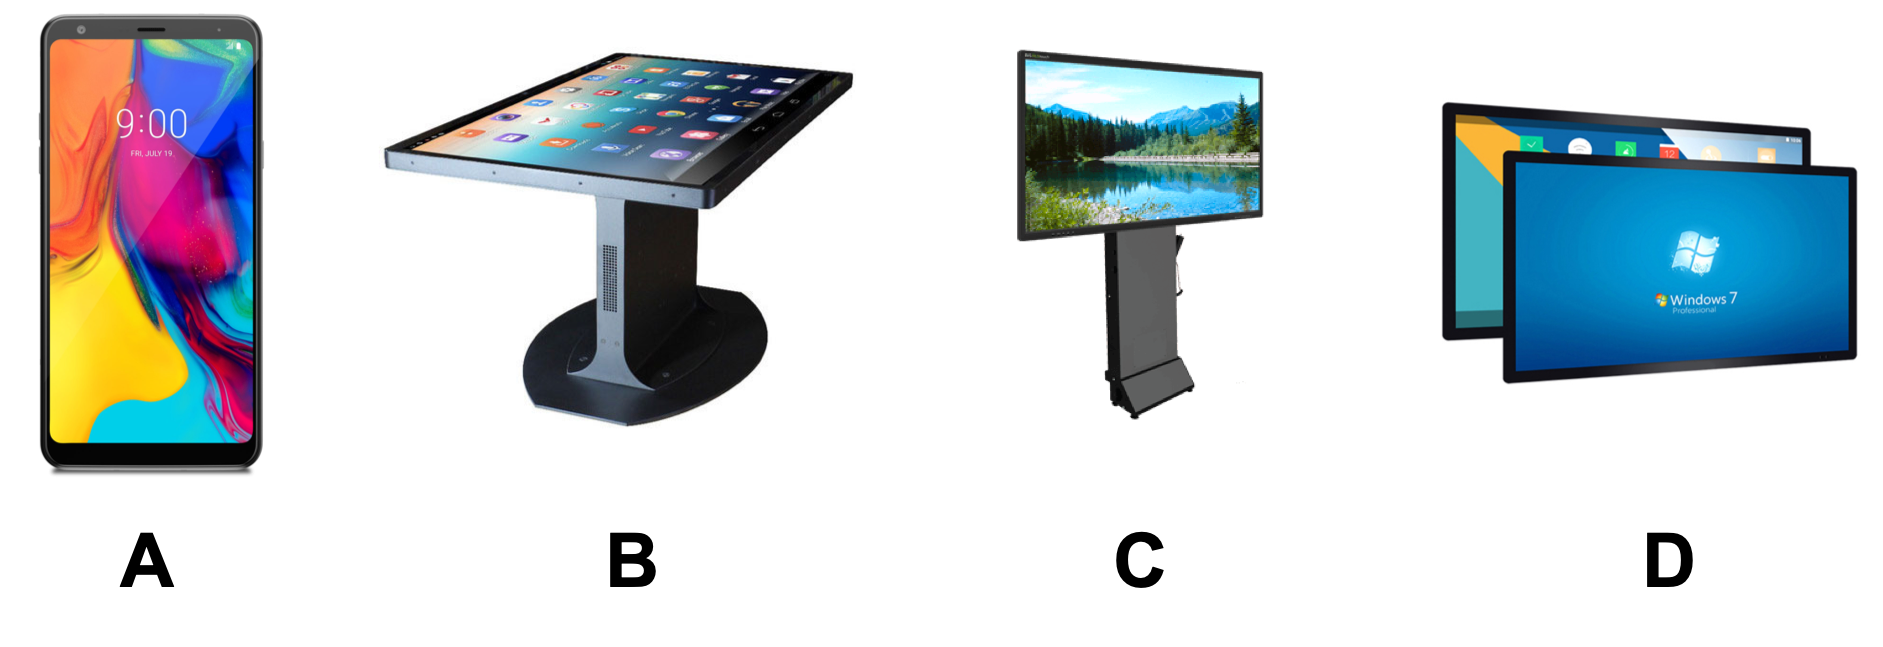
\includegraphics[width=0.95\columnwidth]{figures/touchproducts.png}
    \setlength{\belowcaptionskip}{-8pt}
    \caption{Capacitive touchscreen products: iphone (A). multitouch arcade touchscreen game table (B) interactive whiteboard (C). touchscreen Wall (D).}
    \label{fig:touchscreen-products}
\end{figure}

Researchers have explored enabling touch interfaces on everyday surfaces or objects ~\cite{Ono-Touch-and-Activate, Ono-2014,Sato-Touche, Xiao-WorldKit, Rekimoto-SmartSkin, olberding2013cuttable, Zhang-Electrick} with various sensing techniques. However, to recognize the touch events on everyday objects such as toys, it requires different embedded sensors, such as resonate sensor, capacitive touch sensor, volatage sensor, and camera. 

As we can see, these prior works require dedicated sensing platforms such as Arduino to power touch interfaces and to enable wireless communication with digital devices. These requirements prevent end-users from easily fabricating customizable touch interfaces. Users need to dedicately coporate the sensors with the touch interface and need to build companion computer program for event recognition, which significantly raise the barrier for fast prototyping. 

As an alternative, in recent 5 years, researchers are trying to leverage the existing sensors that are available to everyone to empower everyday objects with sensing capability. Thanks to the ubiquity of capacitive touchscreen device such as smartphone, ipad and latop, researchers have proposed extending the capacitive sensing capability of these touchscreen devices to ambient surfaces through conductive strips. These systems can support interactions such as touch widgets ~\cite{Kato2015a,Kato2015,Kato2016}, trackpad ~\cite{mobicom-gao18} as well as tangible interfaces ~\cite{Schmitz2017, Schmitz2018, Chan-CapStones}. However, though these systems is able to provide interaction beyond touchscreen surface, due to the lack of raw capacitance siganl, the smart device fail to distinguish the touch event between on-screen touch and off-screen touch, which will influence user's normal interaction on touchscreen such as click and slide. Additionaly, these approaches can only support applications with very limited sensing range and fabrication materials. Furthermore, the feasibility of long-range capacitive sensing, the design scope, as well as the applications and user case haven't been fully explored.

Our work focuses on two parts: First, we study the feasibility of augmenting the interaction patterns of existing touchscreen device, such as backboard interaction, edge interaction, without disturbing user's on-screen interactions. We demonstrated that by capturing and analyzing the raw capaitance data of touchscreen device such as smartphone, we can configure a special capacitance threshold to accurately seperate on-screen touch event from off-screen touch event. Based on that, we proposed a series of applications to augment user's interaction experience with ambient surfaces of touchscreen devices (Fig ~\ref{fig:small-scale-scenarios}). Second, we dive deeper into the study of large-scale capacitive sensing using existing capacitive touchscreen devices and conductive materials. Our study shows the possibility of large-scale capacitive sensing. We measured the sensing space of smartphone and proposed two major design patterns of touch interface. Furthermore, we presented example interactive applications of our large-scale sensing technique (Fig ~\ref{fig:large-scale-scenarios}), which is a good alternative of existing large-scale interaction devices such as touch table and touchboard.

\begin{figure}
    \centering
      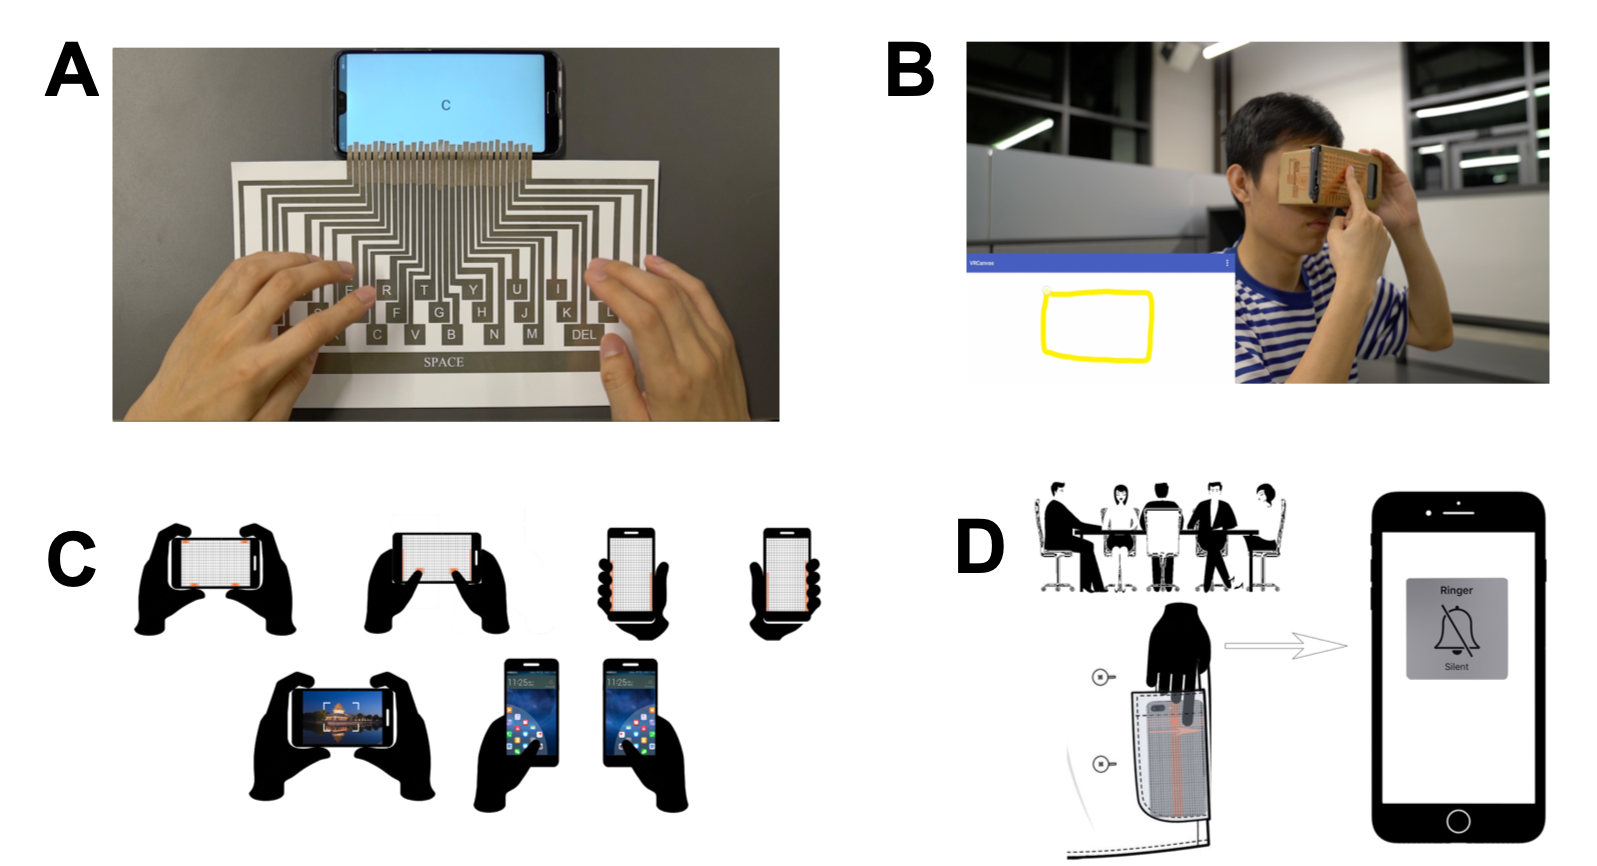
\includegraphics[width=0.78\columnwidth]{figures/small-scale-scenarios.png}
      \setlength{\belowcaptionskip}{-6pt}
      \caption{\textit{FlexTouch} supports ambient interaction around touchscreen device surface. A: Full-size keyboard using silver nanopartical ink-jet printing. B: Enhanced VR interaction of back of smartphone. C: Gesture sensing on edge of smartphone. D: Touch interaction on back of smartphone.}
      \label{fig:small-scale-scenarios}
\end{figure}

\begin{figure}
\centering
  \includegraphics[width=0.9\columnwidth,height=0.4\columnwidth]{figures/scenarios-ubicomp.png}
  \setlength{\belowcaptionskip}{-6pt}
  \caption{\textit{FlexTouch} supports various large-scale applications with different configurations. A: Discrete and 1-dimension touch widgets sensing long-range touch events. B: Fitness tracking using designs in A for the count of repetitions, distance and speed measurement on a treadmill, cycling and chest exercise machine. C: Body posture detection on the yoga mat with a built-in capacitive sensing matrix in an X-Y layout. D: Smart desk application for object presence and user's state detection. E. Smart mattress for sleep monitoring with a one-on-one mapping node matrix from the touchscreen.}
  \label{fig:large-scale-scenarios}
\end{figure}

\section{Thesis Structure}
In this paper, we present \textit{FlexTouch}, a technique for distinguishing off-screen touch from on-screen touch as well as enabling long-range touch sensing interfaces beyond commercial touchscreens by leveraging a variety of flexible conductive materials (Fig ~\ref{fig:small-scale-scenarios}, Fig ~\ref{fig:large-scale-scenarios}). \textit{FlexTouch} utilizes simple fabrication techniques to create a variety of passive, conductive 2D-patterned touch interfaces that enable new health and wellness applications.

In chapter 2, we will introduce related work that is relevant to \textit{FlexTouch}. First, we gathered the current literature aiming at enabling touch interaction on everyday surfaces and objects, including both small-scale and large-scale. We will introduce some techniques these papers applied such as capacitive sensing, volatage sensing, camera sensing, etc. Then we review some work specifically relevant to capacitive sensing beyond touchscreen surfaces. Finally, we discuss the limitation of prior work regarding capacitive sensing and room for innovation and improvement.

Chapter 3 lays out the theoretical principal of 2D capacitive sensing. We present equivalent circuit to explain the effect of attaching conductive materials on touchscreen as well as the effect of off-screen finger touch. Then we elaborate the reason why large-scale capacitive sensing is so difficult and why introducing local ground will amplify the capacitance signal. Based on the equivalent circuit, we give a reasonable assumption that the mutual capacitance scales with the area of extended conductive materials.

Chapter 4 first introduces the signal processing algorithm and procedures of recognizing touch event. Then, we propose several different conductive materials as well as fabrication methods for \textit{FlexTouch} implementation. In particularly, we design a clip-on widget, which we called \textbf{plug and play} interface,  that is able to connect the touchscreen with large interactive surface using copper foil tape.

Chapter 5 conducts a series of evalutaion of \textit{FlexTouch}. The first experiment we conduct is observing the difference of signal pattern between on-screen and off-screen touch. Then we explore the relationship between sensing range and coverage area with different conductive materials, hardward and local ground. To step further into studying the effect of grounding strip, which includes the gap between grounding and signal strip, the width of grounding strip, and the conductivity of grounding strip. Finally, to explore the possibility of detecting the presence of everyday objects, we also evaluated the signal variance of touch event across different objects.

In chapter 6, we focus on real-word applications of \textit{FlexTouch}. The applications of \textit{FlexTouch} can be categorized into two different divisions. The first is what we called \textbf{touchscreen ambient interaction}, second is \textbf{larage-scale extendable interaction}. In the first set of applications, we propose four different scenarios, that are direct augmentation of existing touch interactions around smartphones, such as hold-gesture sensing, backboard touch sensing, external plugin flexible keyboard and VR cardboard interaction. In the second part, we present also four common use cases including smart mattress, yoga mat fitness posture detection, fitness tracking, and smart desk. Additionally, we also conduct concrete user study and quantitative analysis on each application to guarantee the feasibility and robustness of \textit{FlexTouch}.  

As a summary of this paper, chapter 7 concludes our work on extending sensing capability of touchscreen surfaces and potential applications. Fianlly, it points out the future direction of our work from three perspectives.

\section{Main Contributions}
To summarize, some prior work focuses on enabling touch sensing on everyday objects with both regular and irregular shapes, while external sensors and computational board are necessary. Some other work attempts to leverage capacitive sensors embedded in modern smart devices to enable ambient interaction around touchscreens, but being aware of the fact that these ambient interactions only serve as augmentation or translation of existing on-screen touch, and the interaction area is constrained by the screen size. 


Differing from prior work, we leverage the capacitive sensing capability of existing touchscreen to enable everyday-object sensing, off-screen event detection, and large-scale interaction. Our main contributions in this paper are as follow:

1. We differentiated the off-screen touch from on-screen touch, which enables recognizing user's off-screen touch event without disturbing normal on-screen touch event. 

2. We created techniques that leverage a variety of conductive materials and fabrication methods to customize extensions of touchscreens to support continuous 2D touch on everyday objects and ambient surfaces.

3. We enabled large-scale touch sensing up to 4 meters and objects' presence up to 2 meters away from the capacitive touchscreen to ambient surroundings by including the local ground in the external conductive pattern design. 

4. We demonstrated that \textit{FlexTouch} is easy to fabricate, assemble and use. The 2D circuit-like pattern is compatible with various conductive materials (copper foil tape, silver nanoparticle ink, ITO frames, and carbon paint), as well as fabrication methods (cutting, coating, and ink-jet printing). Furthermore, we proposed two easy attaching and assembling approaches to connect the extension part to touchscreens. 

5. We benchmarked the performance of \textit{FlexTouch} through user studies. In particularly, we fully explored design variables such as materials, extension strips' width as well as gap distance between strips and evaluated their impact on the coverage distance of \textit{FlexTouch}. 

6. We demonstrated the versatility and feasibility of \textit{FlexTouch} through multiple applications such as body posture sensing, object presence detection, enhanced fitness sensing applications, etc.


\chapter{Related Work}
In this chapter, we first review a set of work that aims to enable touch interaction on everyday surfaces and objects. Then we dive deeper into prior work in the field of capacitive sensing closely related to \textit{FlexTouch} to better position our work in the related literature.

\section{Touch Interaction on Everyday Surfaces and Objects}
Researchers have explored various methods and techniques to enable interactive interfaces on everyday surfaces and objects. One popular method to enable touch interactions, as shown in Fig ~\ref{fig:cv-large-scale-interaction} is by projecting 2D user interfaces onto a surface and then recognize user interaction via computer vision technique ~\cite{pinhanez2001everywhere, Fails-2002-Light-Widgets, Wilson-2010-Light-Space, Xiao-WorldKit}. For example, \textit{WorldKit} system makes use of a paired projector and a depth camera to capture user's touch-based interaction on surfaces, enabling people to quickly instantiate any shapes of interface they like. To achieve this, the system also requires preconfiguration of functionality of different locations on the surface. Apparently, these solutions can support large-scale interactions which are suitable for fixed infrastructure. However, its power consumption and form factor still make it hard to fit into everyday mobile scenarios. Furthermore, the cost of the toolkit as well as the difficulty of setup also makes it far way from being popularized to the industry.

\begin{figure}[ht]
    \centering
	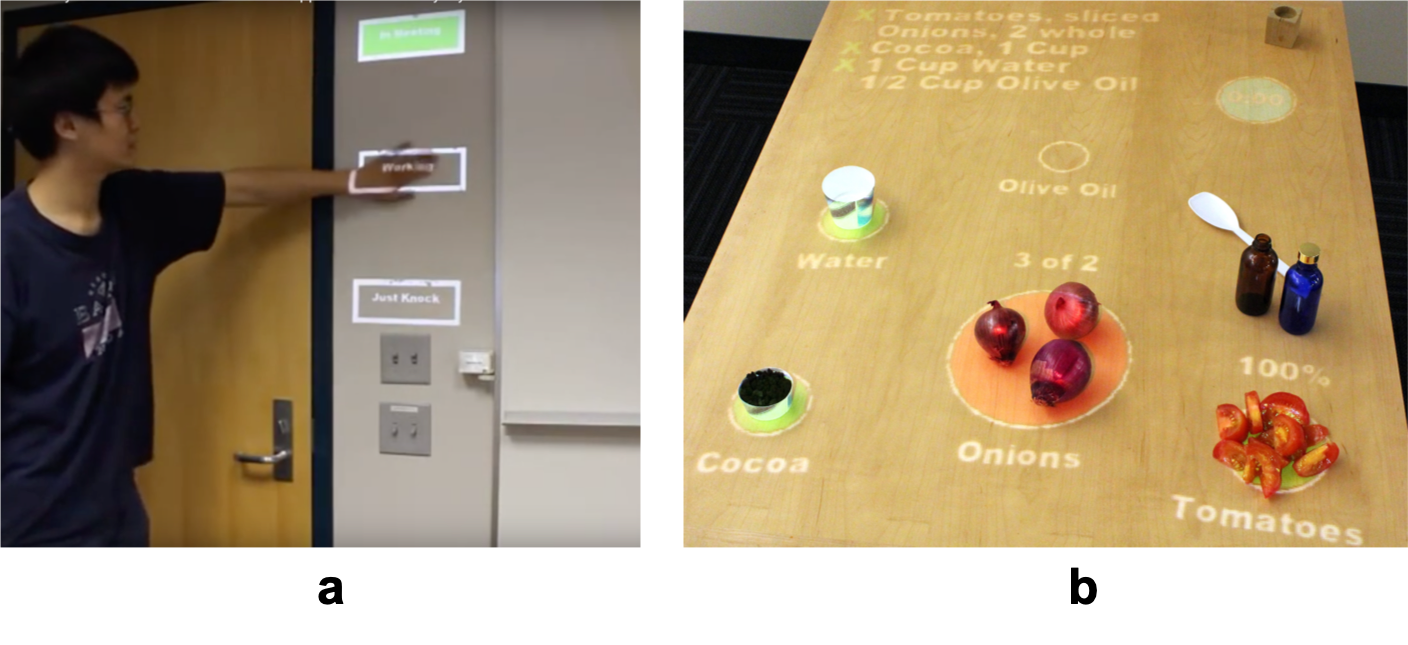
\includegraphics[width=0.78\columnwidth]{figures/cv-large-scale-sensing.png}
	\setlength{\belowcaptionskip}{-6pt}
    \caption{Example applications of vision-based large-scale interaction: a) notification message application. b) Kitchen application.}
    \label{fig:cv-large-scale-interaction}
\end{figure}

Touch interaction can also be supported by acoustic sensing.  Ono's work is based on the difference of resonate properties of different objects ~\cite{Ono-Touch-and-Activate}. As illustrated in Fig \ref{fig:acoustic-sensing}, by attaching a viabration speaker and a piezo-electric microphone, the system collects and amplify the vibration data and transmit it into a computational device. Then, by train a supervised pattern recognition model for recognizing different acoustic wave patterns, it is able to distinguish various touch events. Researchers have also explored recognizing a discrete set of touch events on everyday objects such as windows ~\cite{Paradiso-2002-Window}, desktops, and other surfaces ~\cite{Harrison-2008-Scratch-iput}. However, these approaches only apply towards a small set of touch inputs like tapping or scratching on various materials. Last but not least, these approaches cannot live without dedicated sensing platforms to collect and transmit acoustic data from objects, which adds too much complexity to existing objects.

\begin{figure}[ht]
    \centering
	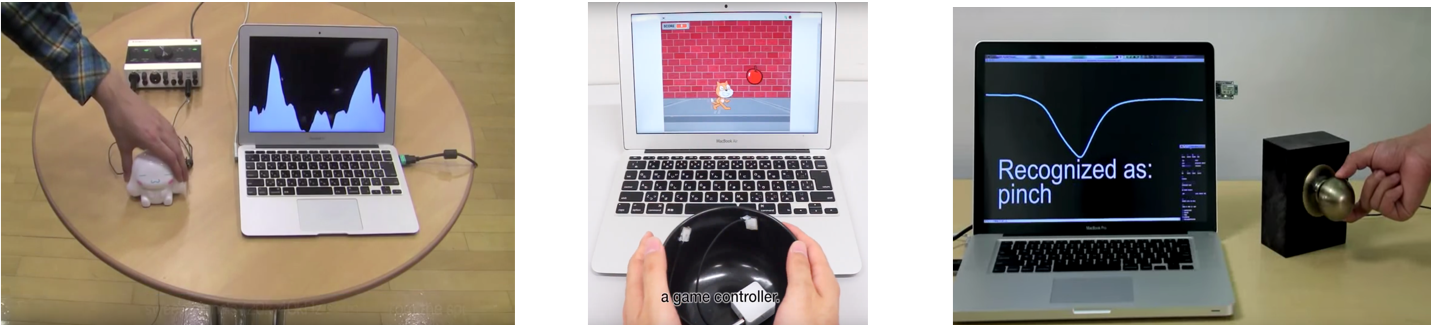
\includegraphics[width=0.88\columnwidth]{figures/acoustic-sensing.png}
	\setlength{\belowcaptionskip}{-6pt}
    \caption{Touch and Activate: Adding interactivity of existing objects using active acoustic sensing}
    \label{fig:acoustic-sensing}
\end{figure}

Another popular method is electromagnetic sensing. \textit{SmartSkin} enabled multi-touch interaction on surfaces using a mesh-shaped capacitive sensor grid ~\cite{Rekimoto-SmartSkin}. They make use of a capacitive sensor grid with size of 32 \times 24 to detect touch events on a large-scale surface. 
\begin{figure}[ht]
    \centering
	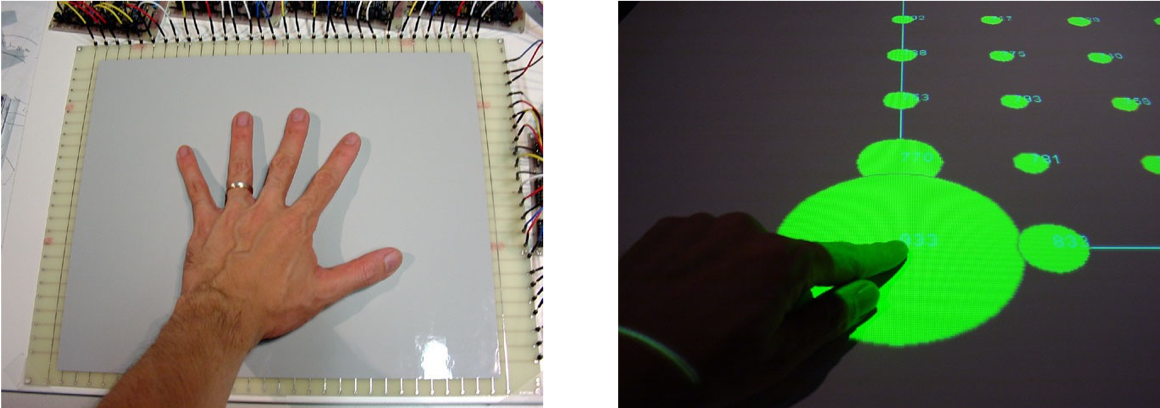
\includegraphics[width=0.88\columnwidth]{figures/smartskin.png}
	\setlength{\belowcaptionskip}{-6pt}
    \caption{\textit{SmartSkin} is embedded with dense capacitive sensors to achieve accurate touch sensing on flat surface.}
    \label{fig:smartskin}
\end{figure}

\textit{Electrick} ~\cite{Zhang-Electrick} and \textit{Pulp Nonfiction} ~\cite{Zhang-pulp} enabled touch input on everyday surfaces and objects using Electric Field Tomography (EIT) with coated conductive materials on everyday surfaces and objects. As shown in Fig ~\ref{fig:electrick}, by sensing the voltage difference between paired electrodes before and after touch, \textit{Electrick} can accurately locates user's touch position as well as measuring the pressure of touch event. 

\begin{figure}[ht]
    \centering
	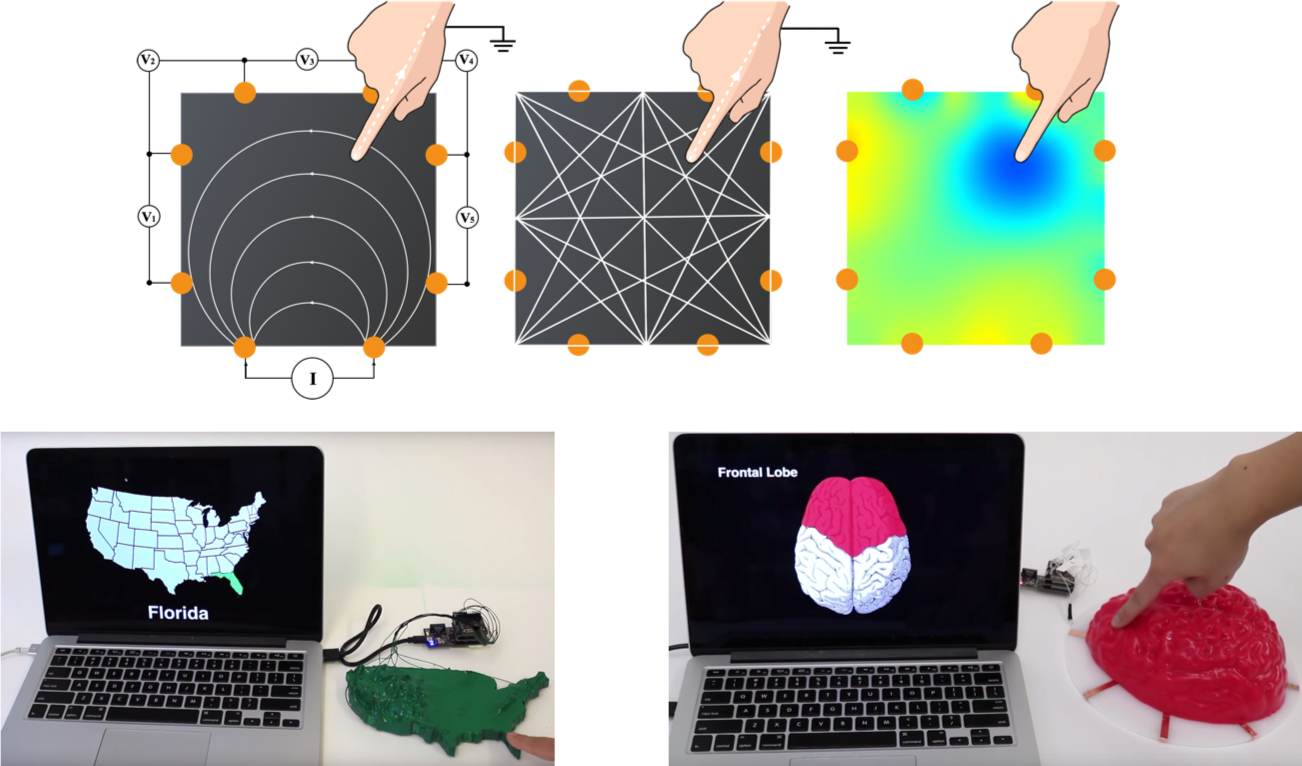
\includegraphics[width=0.88\columnwidth]{figures/electrick.png}
	\setlength{\belowcaptionskip}{-6pt}
    \caption{\textit{Electrick}: Enabling low-cost touch sensing on any shapes of surfaces by using electric field tomography}
    \label{fig:electrick}
\end{figure}

\textit{Touche} ~\cite{Sato-Touche} enhances touch interface on the human body or everyday objects by measuring the electrical profiles with a frequency-sweep signal. \textit{Midas} ~\cite{Savage-2012-Midas} fabricated customized capacitive touch sensors to prototyping interactive object with a circuit board milling machine. \textit{Cuttable} ~\cite{olberding2013cuttable} goes a big step further in customization, which allows customizable shapes of sensor by cutting. \textit{Wall++} ~\cite{Zhang-wall} enabled large-scale touch interaction on the wall for activity recognition. Other prior work also explored printing custom-shaped capacitive sensors ~\cite{gong2014printsense,olberding2015foldio,olberding2014printscreen,vadgama2017flexy}. These prior works demonstrated very promising results, again however, they rely heavily on dedicated sensing platforms and customized embedded systems to provide power supply, external sensors, signal processing, and communication modules. These requirements create barriers for end-users to easily fabricate customized touch interfaces.

\begin{figure}[ht]
    \centering
	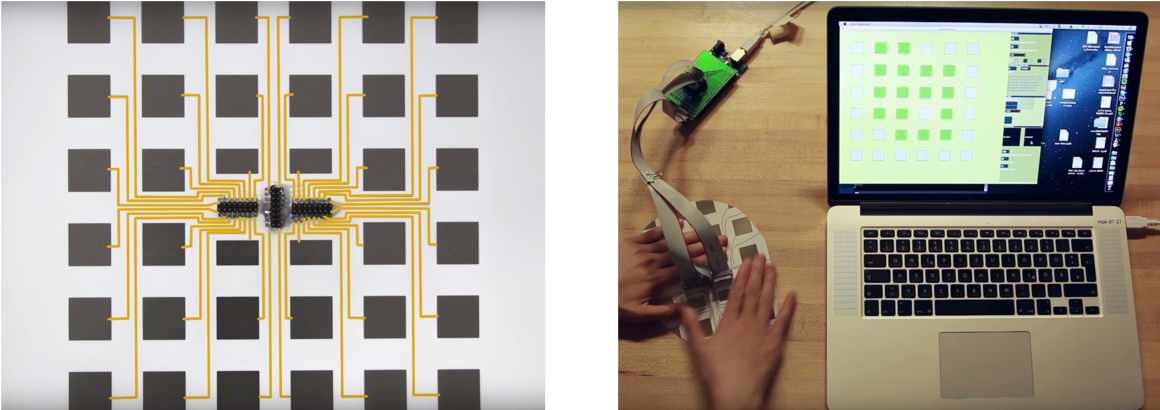
\includegraphics[width=0.88\columnwidth]{figures/cuttable.png}
	\setlength{\belowcaptionskip}{-6pt}
    \caption{A cuttable multitouch sensor using tree topology electrodes and flexible materials.}
    \label{fig:cuttable}
\end{figure}



\section{Capacitive Touch Interaction Sensing beyond Touchscreens}
Capacitive sensing was introduced into the field of HCI over two decades ago. Recently, Grosse-Puppendahl and his colleagues reviewed and summarized past researches related to capacitive sensing theories and techniques ~\cite{Grosse-Puppendahl-capacitive}. Among all the capacitive sensing methods, shunt mode sensing is the most widely spread approach in implementing modern capacitive touchscreens. The touch panel consists of multiple layers above the display screen with all the sensing nodes oriented in a row-column matrix (Fig ~\ref{fig:multi-layer-touchscreen}). Each node is a high-resolution continuous capacitance measurement sensor. Obtaining the low-level capacitive data from the touchscreen provides us with more capability beyond binary finger touch sensing. 

\begin{figure}[ht]
    \centering
	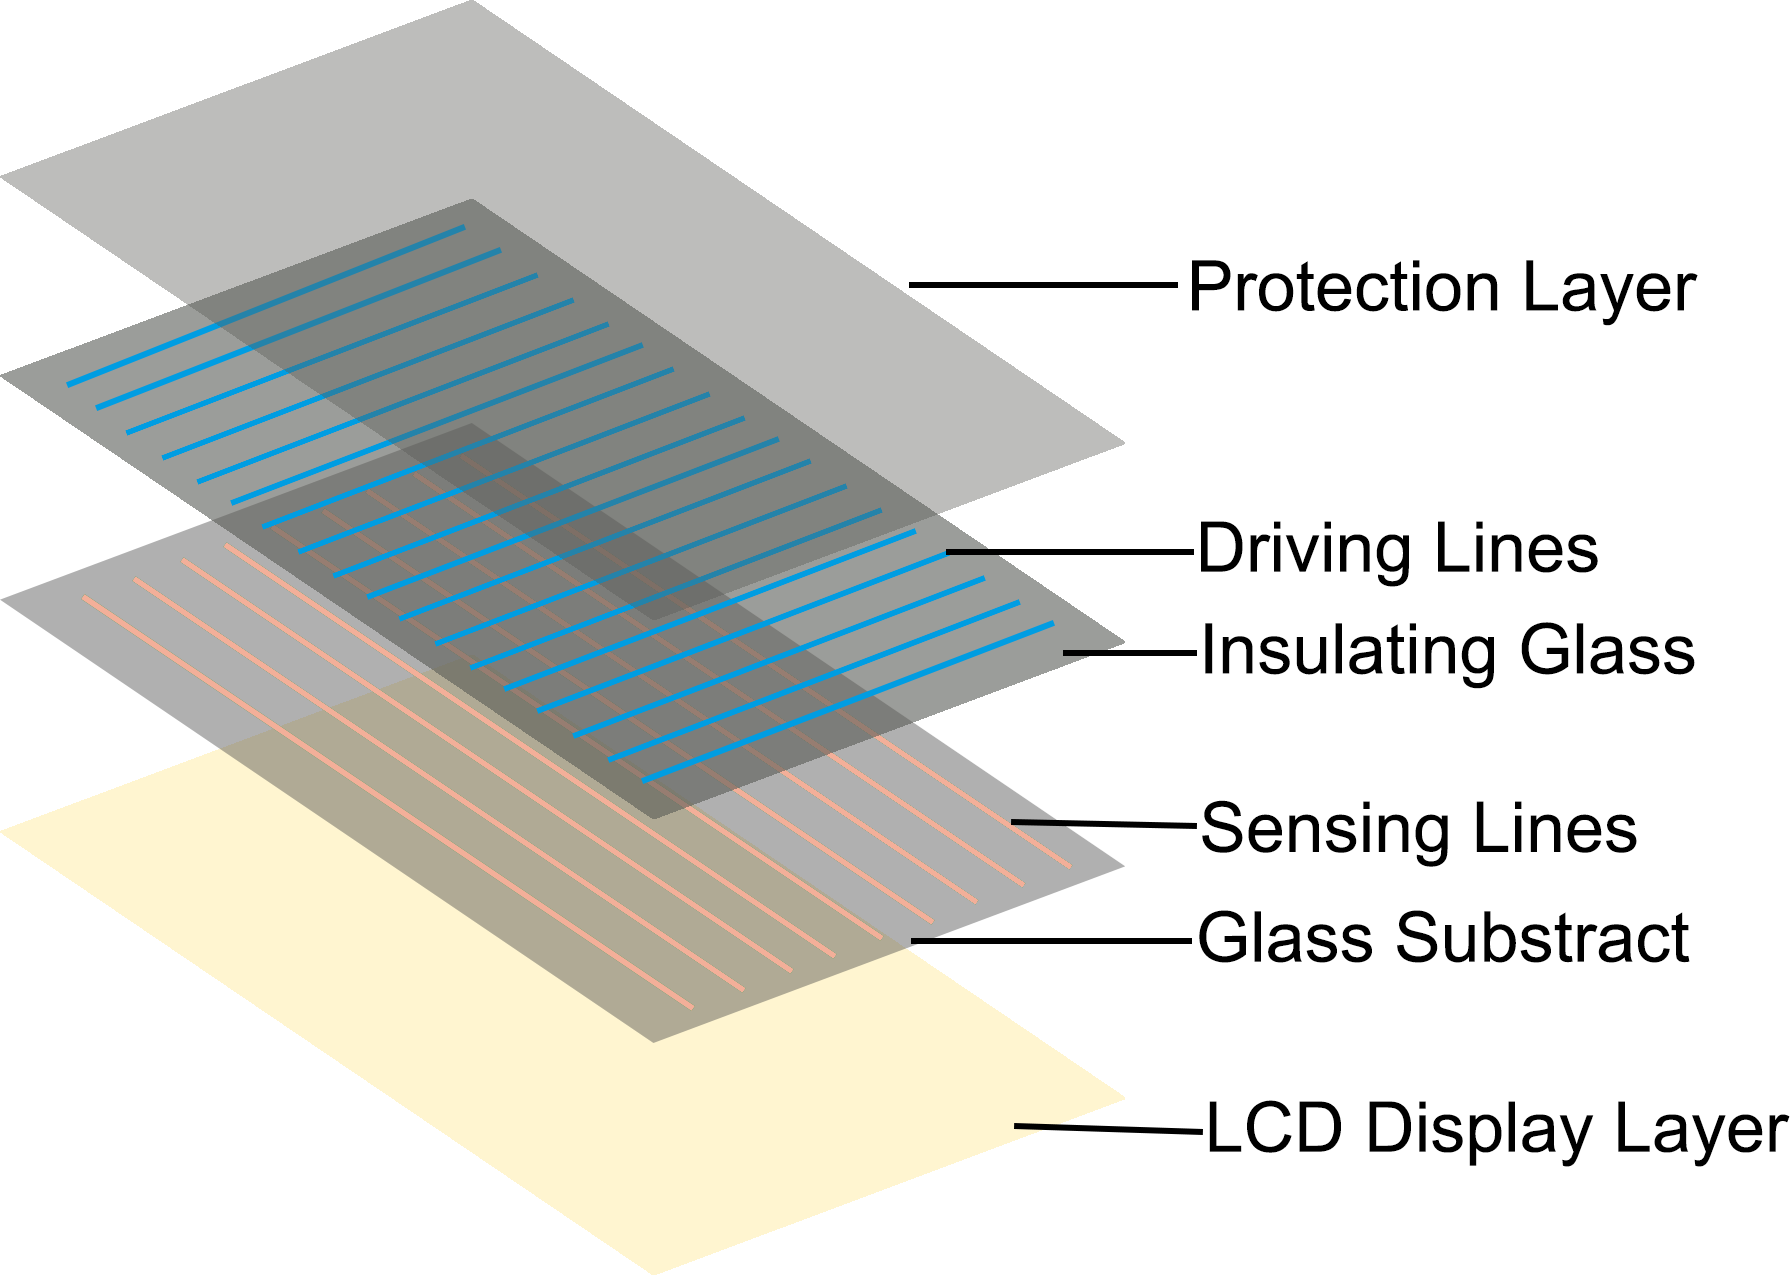
\includegraphics[width=0.78\columnwidth]{figures/multi-layer-touchscreen.png}
	\setlength{\belowcaptionskip}{-6pt}
    \caption{The multi-layer structure of mutual capacitance touchscreen. }
    \label{fig:multi-layer-touchscreen}
\end{figure}

Similar to our approach, \textit{BodyPrint} ~\cite{Holz-bodyprint} and \textit{CapAuth} ~\cite{Guo2015} (Fig ~\ref{fig:capacitive-auth}) combined capacitive touchscreens with machine learning classifiers to provide authentication and even identification of users by recognizing different patterns of capacitance image on touchscreen. \textit{PalmTouch} enabled the palm as an additional input modality to enhance mobile interaction ~\cite{Le-palmtouch}. Researchers also explored the potential of using the raw capacitive data of touchscreens to support sensing of tangible 3D-printed gadgets on top of the screen ~\cite{Chan-CapStones, Schmitz2017, Schmitz2018}. While these prior works share the same raw capacitance signal as our approach, we focus on fabricating conductive interfaces to support large-scale, flexible touch interfaces on the ambient surfaces connected to touchscreens.

\begin{figure}[ht]
    \centering
	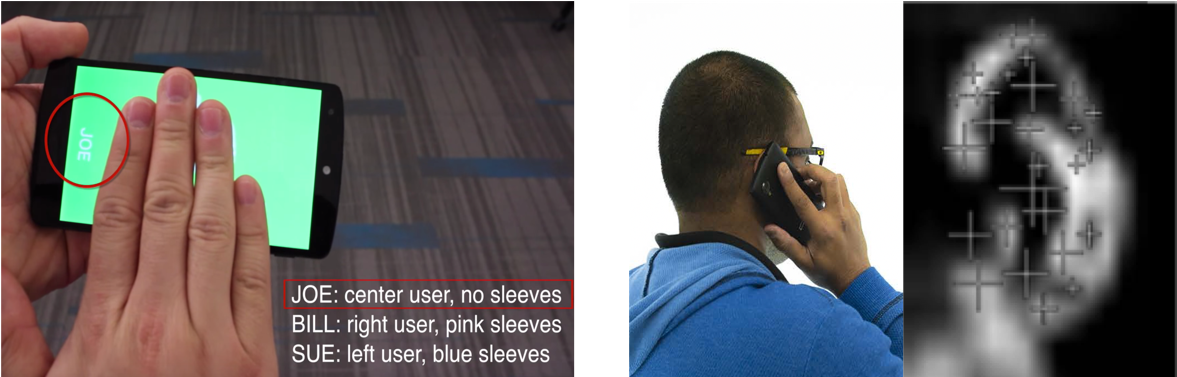
\includegraphics[width=0.88\columnwidth]{figures/capacitive-auth.png}
	\setlength{\belowcaptionskip}{-6pt}
    \caption{User authentications using capacitive sensors on touchscreen.}
    \label{fig:capacitive-auth}
\end{figure}

Modern mobile devices are embedded with rich sensors and actuators. Researchers have explored approaches and techniques enhancing the interaction around mobile devices with customized sensors via active and passive techniques. Researchers have explored attaching capacitive sensors to mobile devices to enable interactive user applications. iGrasp ~\cite{Cheng2013a} and IrotateGrasp ~\cite{Cheng-2013-IrotateGrasp} used capacitive touch sensors on the edge and back of the mobile device to recognize the hold postures for adaptive keyboard layout and screen rotation. These approaches demonstrate promising applications space, however, the requirement of external sensors, power source and processing unit create barriers for massive adoption.

Researchers also explored leveraging the built-in sensors to enhance the interaction on or around the touchscreen. Acoustruments ~\cite{laput2015acoustruments} constructed various sensing units that can detect hand interaction around mobile devices such as touch, proximity and rotation by measuring the acoustic signal transmitted in an enclosed, pipe-like pathway from the speaker to the microphone. UbiTouch ~\cite{wen2016ubitouch} enabled touch interface on surrounding surfaces using build-in proximity and ambient light sensors. Wang and colleagues presented a virtual keyboard technique on the surrounding surface of mobile devices through harnessing multipath fading with multiple built-in microphones ~\cite{wang2014ubiquitous}. 

In close proximity to our work, researchers explored methods extending touch interaction from the touchscreen to ambient objects or surfaces with conductive materials. \textit{Clip-on Gadgets} extended capacitive touchpoints on the phone to physical controllers via conductive materials ~\cite{Yu2011}. Kato and his colleagues went a step further, fabricating 3D-printed conductive gadgets with haptic feedback patterns ~\cite{Kato2016}. User interaction with these gadgets was detected via the capacitive screen when they were placed onto the phone. In addition, they also presented a technique named \textit{ExtensionSticker} which allowed touch sensing to be transferred to ambient surfaces ~\cite{Kato2015, Kato2015a}. However, without accessing the raw capacitive data, \textit{ExtensionSticker} could not support large-scale touch interfaces. Long-range conductive strips attached on touchscreens would be recognized by the built-in touch detector as finger touch events, which prevents the detection of real touches on the strip. As a result, these extension-sticker techniques only allow for near-range touch sensing interfaces. Recently, Gao and Ikematsu demonstrated the feasibility of using 1D conductive ink strips or ABS filament arrays sensing 2D finger positioning ~\cite{mobicom-gao18, Ikematsu-Ohmic-Touch} through measuring the resistance introduced to the touchscreen's sensing circuit. However, they only demonstrated short-range applications such as 2D finger tracking on phone-based VR headsets or 1D touch bar using a single sensor node. Though these work already provides diverse interaction surrounding smartphone, they are not able to differentiate off-screen touch and on-screen touch. In some cases when user is conducting on-screen touch, it is possible for the smart device to mistakenly recognize the event as off-screen touch due to the similarity of capacitive image pattern.

\begin{figure}[ht]
    \centering
	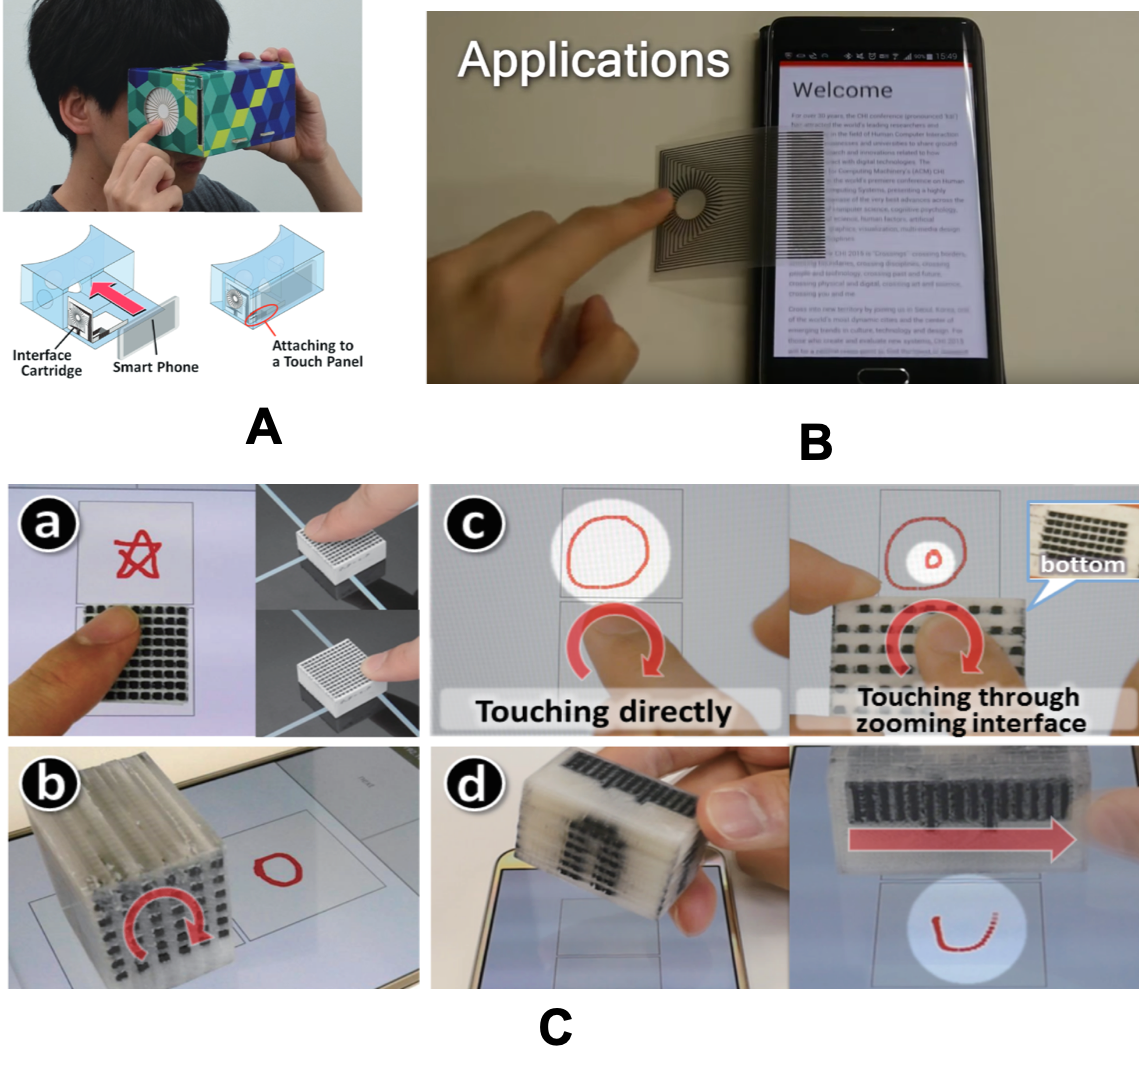
\includegraphics[width=0.88\columnwidth]{figures/ambient-capcitive-sensing.png}
	\setlength{\belowcaptionskip}{-6pt}
    \caption{Extending touch interaction to ambient objects using strip-like conductive materials. A: Mobile head-mounted display with proprietary controller. B: Smartphone side-input controller. C: Conductive gadget that enables touching, zooming and sliding interaction.}
    \label{fig:ambient-capcitive-sensing}
\end{figure}

In contrast with prior work, \textit{FlexTouch} can perfectly differentiate on-screen touch from off-screen touch based on our study of raw capacitance signal of these two interaction modes. More importantly, \textit{FlexTouch} allows users to create large-scale, passive, flexible and customizable touch sensitive gadgets that can be easily attached to the mobile touchscreen for rapid prototyping of interactive applications. To further empower large-scale capacitive sensing, we leverage the local ground plane of the touchscreen to boost capacitance signal strength that enables touch-sensing coverage range up to 4 meters and objects' presence sensing range up to 2 meters, which we think is a significant milestone in large-scale touchscreen-based capacitive sensing. This capability allows \textit{FlexTouch} to support large-scale sensing applications such as touch sensitive yoga mats or bed mattresses with signal processing and machine learning techniques. These advancements provide \textit{FlexTouch} with potentials to be applicable to a variety of new touch sensing applications beyond prior works.

\section{Summary}
In this chapter, we walked through the body of literature related to our work, and introduced several different touch sensing techniques, ranging from acoustic sensing, electromagnetic sensing to capacitive sensing, that are applied to augment the interactivity of everyday surfaces and objects. Some work already supports large-scale touch sensing, but dedicated sensing platform and external power are essential to these systems. Then we took a closer look at capacitive sensing beyond touchscreens. We introduced some work that innovatively leverage the embedded sensors in smartphone for user authentications. Coupled with smartphone, well-designed touch interface like \textit{ExtentionSticker} and conductive gadget make full use of touchscreen that provide user with a more natural and efficient way of basic interactions around smartphone. However, these interactions are only augmentation or a form of translation of on-screen touch, which heavily relies on existing touch events such as click, and does not allow user to define customizable off-screen interaction. Finally, we introduced our work \textit{FlexTouch}, which specifically solve the off-screen detection problem as well as interaction scaling problem.
\chapter{FlexTouch Working Principles}

\section{Sensing Principle of Touchscreen}
Most touch screens today are based on either self or mutual capacitive touch sensing. The mutual capacitive touch sensing method is widely adopted in industry due to its robustness in sensing multiple touch points simultaneously ~\cite{ye2015high}. The touch panel consists of multiple layers above the display screen as demonstrated in Figure ~\ref{fig:multi-layer-touchscreen}. A substrate glass etched with the sensing lines is attached. Then a layer of insulating material etched with the driving lines is placed on top. Finally, a bonding layer and a protective layer are placed on the top of the stack. 

The driving and sensing lines are made by a highly transparent conductive material named Indium Tin Oxide (ITO). They are oriented in a row-column matrix. A thin insulating layer between the driving lines and sensing lines forms a gap, the coupling mutual capacitance is formed at each junction (intersection between the driving and sensing lines) \cite{barrett2010projected}. Dedicated IC drives each driving line (row) and scans all the the sensing lines (columns) to measure the capacitance value at each row-column intersection. This procedure is repeated for all the driving lines as one entire cycle as Figure ~\ref{fig:touchscreen-principle-circuit} A) shows. 

\begin{figure}[h]
\centering
  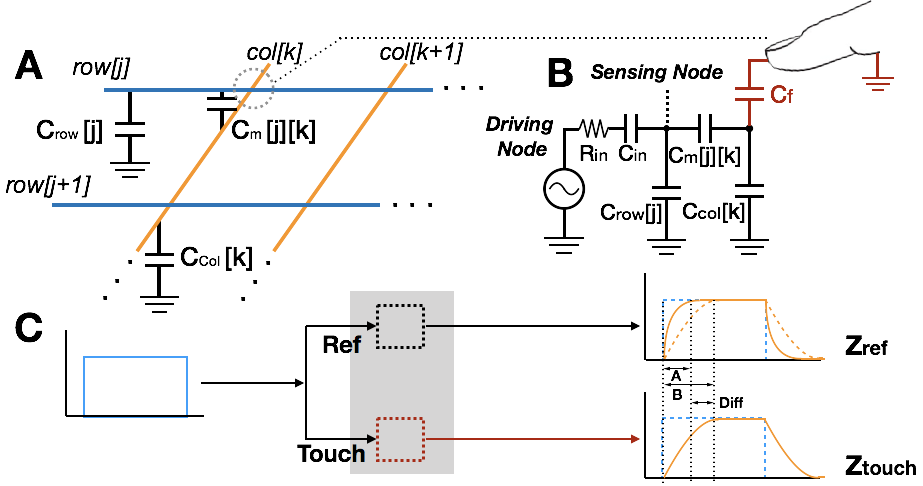
\includegraphics[width=0.95\columnwidth]{figures/touchscreen-principle-circuit.png}
  \caption{A: Representation of capacitive sensing row-column matrix structure B: Equivalent circuit of each junction. C: The measurement of capacitance of each junction.}
  \label{fig:touchscreen-principle-circuit}
\end{figure}

The finger touch increases the mutual capacitance of the touched electrodes. To detect the touch events, the driver IC measures the capacitance of each electrode intersection by comparing the source signal injected to the driving line and returned signal from the sensing line. The equivalent circuit and measuring method are illustrated in Figure ~\ref{fig:touchscreen-principle-circuit} B) and C). The standard method to detect the mutual capacitance of each junction is to measure the charging time to reach a certain voltage threshold between the driving line and the sensing line. 

\section{FlexTouch}

\textit{FlexTouch} extends the capacitive sensing method of commercially available touch screen to surrounding areas through a single conductive thread or frame attached on each sensing electrode. The attached conductive material, changes the electric field around the capacitive sensing junction. In this section, we explain the working principle, implementation and various of design configurations of \textit{FlexTouch}.

The conductive thread attached onto the touch screen draws currents passing from the driving line around the corresponding junctions. As a result, it takes more time to charge both the inner circuit and the attached conductive thread. In other words, any attached conductive material increases the mutual capacitance of the capacitive sensing node. Consider another case when people touch on the conductive thread, human body draws additional currents from the touch screen that further increases the mutual capacitance. In Figure ~\ref{fig:flextouch-principle-circuit} ,the measurement output from each junction node is positively correlated to mutual capacitance. In Figure  ~\ref{fig:flextouch-principle-circuit}A, the measurement of junction \#16 is 2 when no finger touch is present and now conductive thread is attached. When we connect an copper conductive thread onto the sensing node, the measurement jumped up to 983. And when a user is pressing onto the thread, the measurement is further increased to 1090 accordingly. If user press on both signal strip and grounding strip, the signal significantly increase to 1453, which demonstrated the amplifying effect of grounding strip.

Any conductive object in contact with the touchscreen draws currents passing from the driving line (transmitting electrode) to the sensing line (receiving electrode) at each junction. The control IC of the touchscreen is designed to measure this leaking current to detect touch events. Prior work introduced an extension tape enlarging the transmitting electrode to boost the touch sensing distance ~\cite{Kato2015, Kato2015a,mobicom-gao18, Ikematsu-Ohmic-Touch}. In Kato's work, the signal transmitted into the conductive tape returns to the device through an environmental coupling path, called \textbf{\textit{virtual ground}}. To further extend the capacitive sensing distance, we introduce the ground of the phone, the \textbf{\textit{local ground}}, into the extended circuit. Therefore, we can short this coupling path with another conductive tape directly passing the signal back to the touchscreen device. Although the local ground can be extended from the charging port, we use the back panel of the touchscreen device since it's easier to assemble as illustrated in Fig ~\ref{fig:plugandplay} C. We can simplify the structure made of the attached conductive tape, the back panel, and the inner local ground circuit as one large capacitor. Here, we define two types of extension strips: 1) \textbf{\textit{signal strip}}, which is attached to the touchscreen sensor node, and 2) \textbf{\textit{grounding strip}} which extends the local ground of the touchscreen.

\begin{figure}[ht]
\centering
    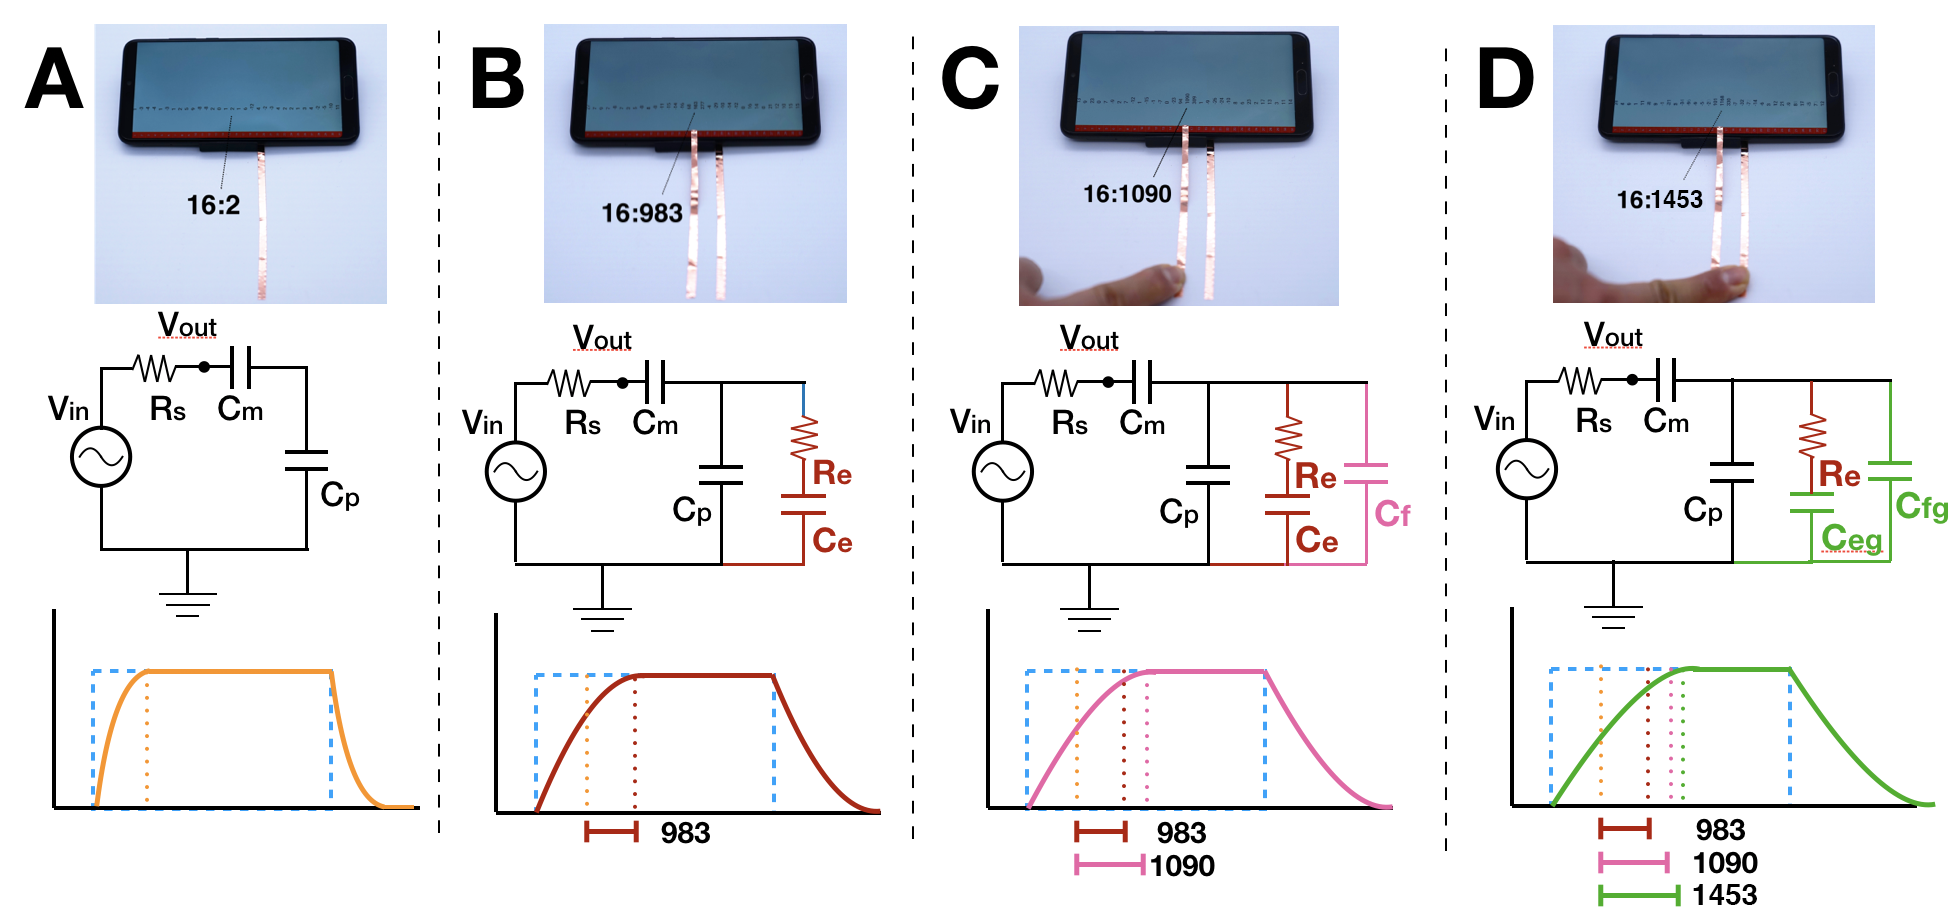
\includegraphics[width=0.95\columnwidth]{figures/flextouch-principle-circuit.png}
    \setlength{\belowcaptionskip}{-6pt}
    \caption{Four capacitive states and corresponding simplified equivalent circuits of \textit{FlexTouch}. A: Idle state - original touchscreen sensing node. B: Attaching state - adding the signal strip on one touchscreen sensing node. C: Touching state - touch on the signal strip. D: Grounding state - touch both the signal strip and the grounding strip.}
    \label{fig:flextouch-principle-circuit}
\end{figure}

We present simplified equivalent circuits under each column in Fig ~\ref{fig:flextouch-principle-circuit} with each capacitive sensor node treated as a RC circuit. $R_{s}$, $C_{m}$, $C_{p}$, $C_{e}$, $C_{f}$, $C_{fg}$,$C_{eg}$, $R_{e}$ represent the inner resistance, mutual capacitance, parasitic capacitance, introduced capacitance between the extended element and local ground, touch introduced capacitance, introduced capacitance of touching both the signal and grounding strips, changed capacitance between the extended element and local ground as well as the extended element introduced resistance. Equation (1) shows the calculation of $v_{out}$ ignoring the effect of $R_{e}$, using $C_{e(g)}$ representing either $C_{e}$ or $C_{eg}$ and $C_{f(g)}$ representing either $C_{f}$ or $C_{fg}$.

\begin{equation}
    V_{out} = v_{in}(1-e^{-\frac{C_{m} + C_{p} + C_{e(g)} + C_{f(g)}}{R_{s}C_{m}(C_{p} + C_{e(g)} + C_{f(g)})}t})
\end{equation}


The touchscreen controller transmits a series of step voltage signals to scan through each electrode and measures the charging time (time for $V_{out}$ to reach a threshold) as raw capacitive values of the touchscreen. The charging time is linearly dependent on the Time Constant of the RC circuit, named $\tau$, that is given as:

\begin{equation}
    \tau = R_{s}\frac{C_{m}(C_{p} + C_{e(g)} + C_{f(g)})}{C_{m} + C_{p} + C_{e(g)} + C_{f(g)}}
\end{equation}

 
We assume that $C_{m}$ and $C_{p}$ are static with value around $10pF$. The value of $C_{e}$ depends on the characteristics of the extended surfaces such as conductivity of the material, length, and width as well as the intersection effect between the extended elements. $C_{f}$ typically varies from several to dozens of $pF$ introduced by human touch. 

Fully understanding the effect of $C_{e}$ is the key to exploring the upper-limit of \textit{FlexTouch}'s performance. In pursuit of testing this limit, we simply model the mutual capacitance between the extended material and the virtual ground with following formula.

\begin{equation}
    C_{e} = \varepsilon \frac{A}{d} = \varepsilon \frac{L \times D}{d}
\end{equation}

$A$ represents the scale of dimensions of extension strips including length ($L$) and width ($D$), $d$ represents the separation between the signal strip and the local ground, and $\varepsilon$ represents the material's permittivity of extension strips. Therefore, to fully evaluate the sensing distance capability of \textit{FlexTouch}, we need to study the effect of variable factors contained in the fabrication material along with the width and gap distance of the extension strips.

\section{Summary}
In this chapter, we introduced the sensing principles that related to \textit{FlexTouch}. We first briefly talked about the capacitive sensing principle of modern touchscreen. Then we dived deeper into the sensing principle of \textit{FlexTouch} by discussing the equivalent RC circuit in detail. Finally, we conducted a qualitative analysis of \textit{FlexTouch} sensing based on the formulas we derived, which pointed out some factors needed to be studied to figure out the design space of \textit{FlexTouch}. 

\chapter{FlexTouch Implementation}

To validate the feasibility of our approach across different Android devices, We implemented \textit{FlexTouch} on a Huawei P20 and a Huawei P10 phone. By rooting the Android operating system and modifying the driver of the touch screen controller IC in the kernel's source code, we extracted the raw capacitive sensing data: $32 \times 16 = 512 px$ 16-bit diff value image across a 5.8-inch surface at 100 fps for Huawei P20 phone, $28 \times 16 = 448 px$, 16-bit diff value image across 5.1-inch surface area at 20 fps for Huawei P10 phone. We built an Android application that shows positions and raw capacitive values with corresponding update rates of chosen sensing nodes. The app also logs the raw capacitive image to a local server for later analysis.

\begin{figure}[ht]
    \centering
      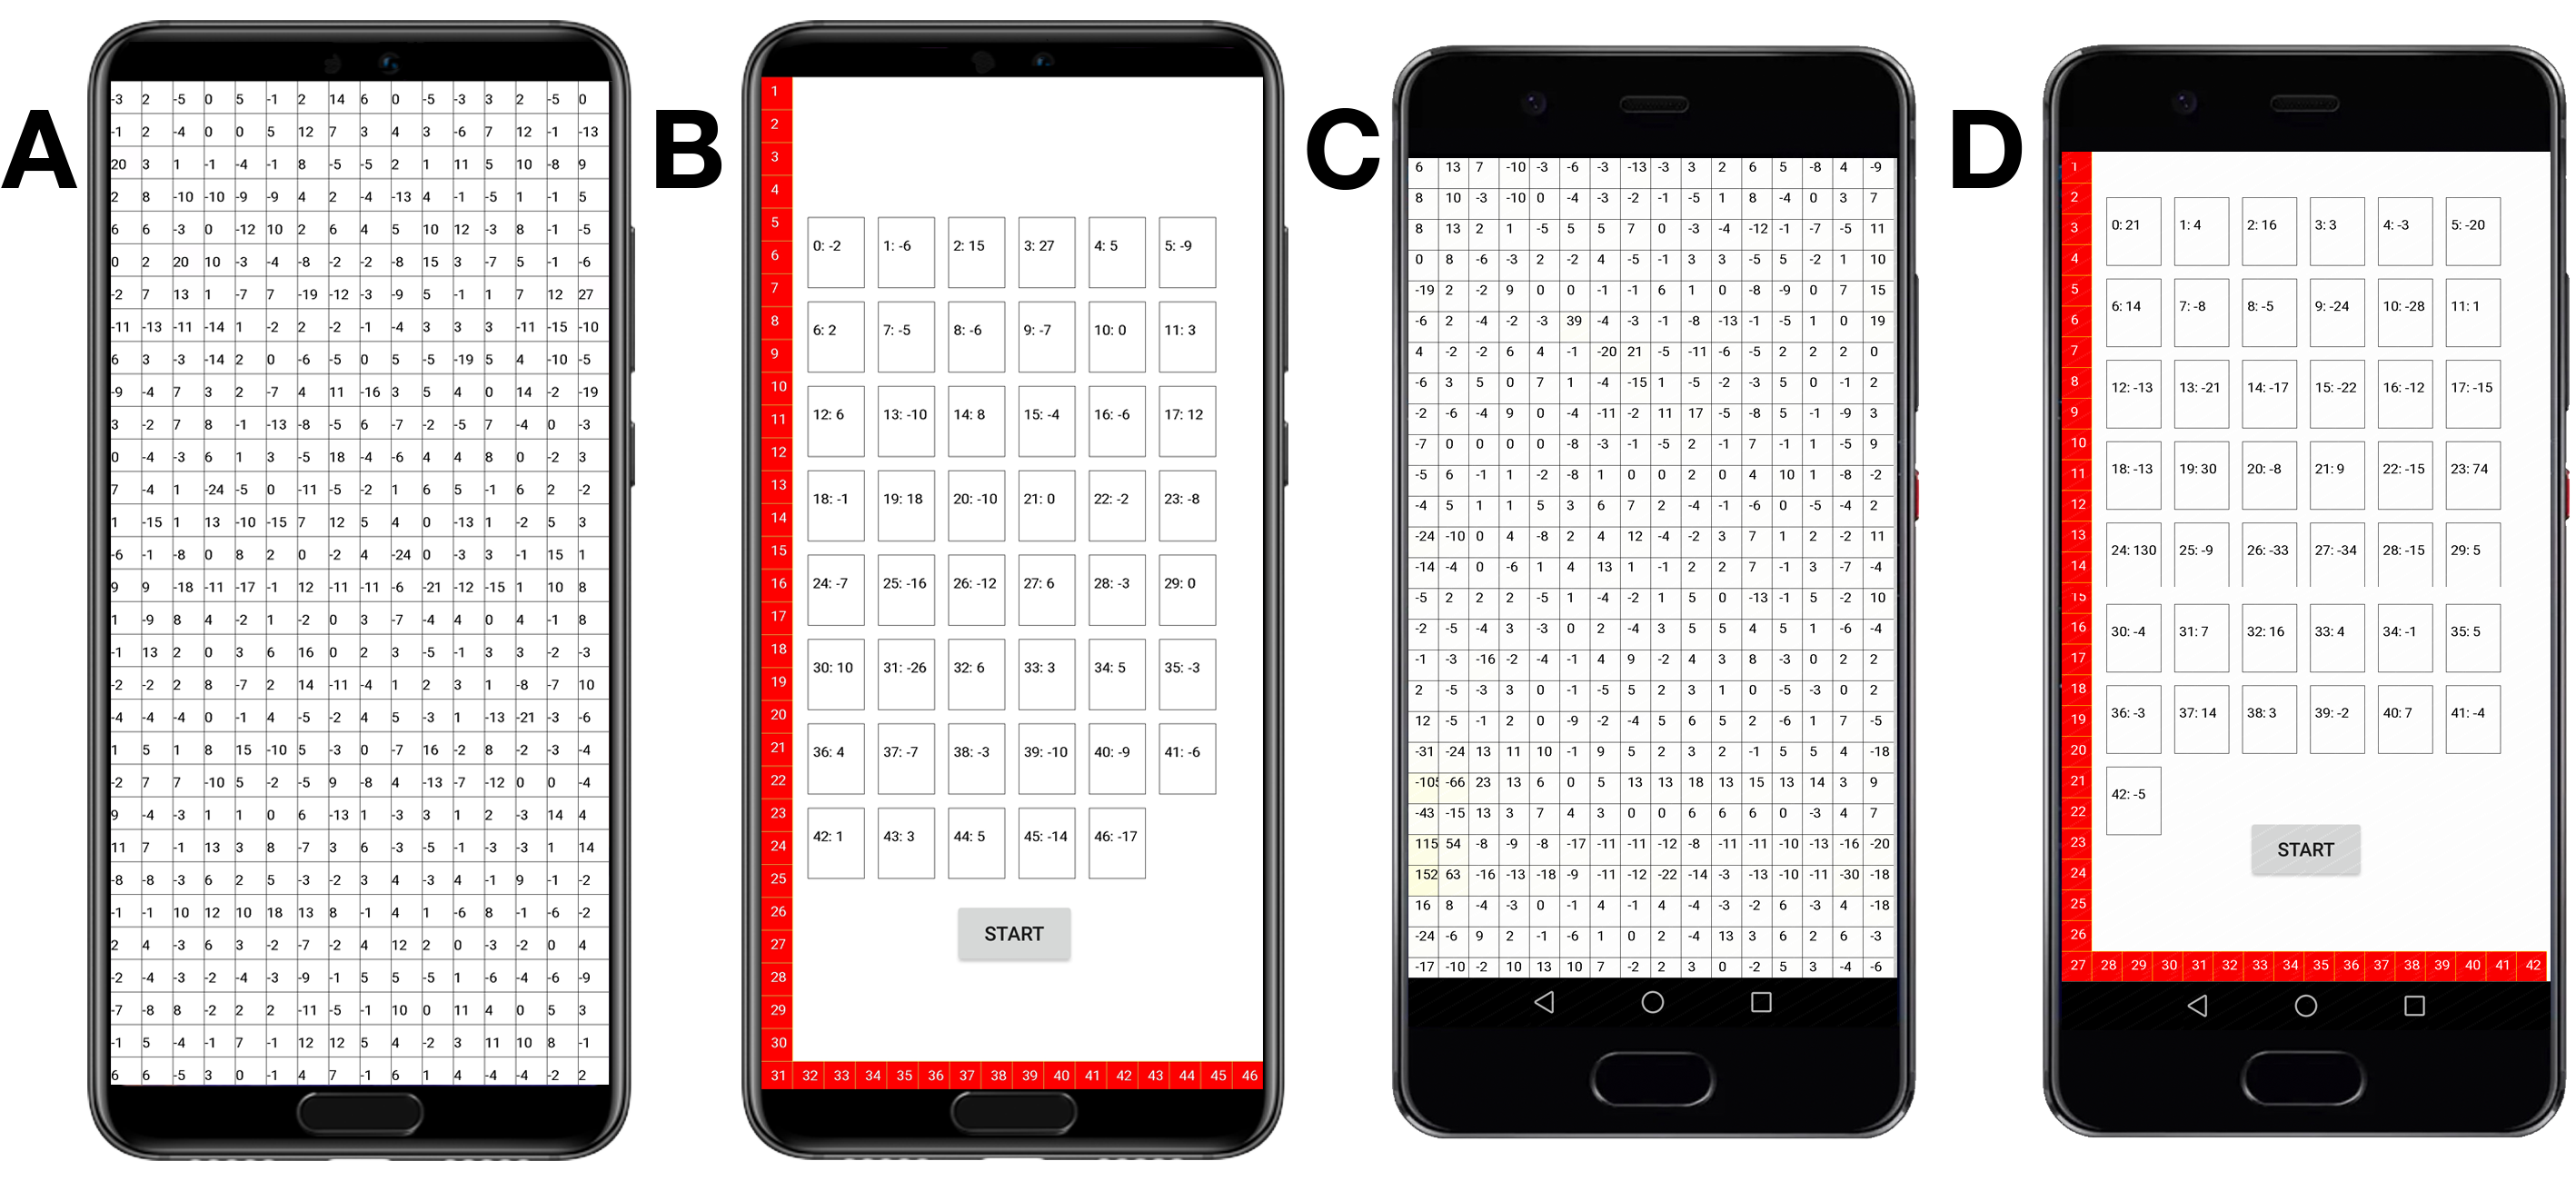
\includegraphics[width=0.95\columnwidth]{figures/rawdata.png}
      \setlength{\belowcaptionskip}{-6pt}
      \caption{Android Applications showing the raw capacitive data and positions of the sensing nodes.}
      \label{fig:Android Applications showing the raw capacitive data and positions of the sensing nodes.}
\end{figure}

\section{FlexTouch Sensing Capabilities}
We summarized the sensing capabilities of \textit{FlexTouch} into four categories as shown in Figure ~\ref{fig:1d2d-principle}. 

a) 1D touch interfaces enable tangible discrete touchable buttons, 1D touch gesture widgets.

b) 2D continuous multi-touch tracking enables large-scale multi-touch tracking or hand/body activity detection. 

c) 2D High resolution single-touch tracking via extending ($N$) capacitive sensing junctions into X-Y matrix configuration that enables $N^2/4$ capacitive sensing nodes. 

d) Everyday object state sensing includes object presence detection and object state sensing based on capacitance measurement. 

Note that sensing capability a) has been discussed in prior work ~\cite{Kato2015}. But the other modalities are unique to \textit{FlexTouch}.

\begin{figure}[h]
\centering
  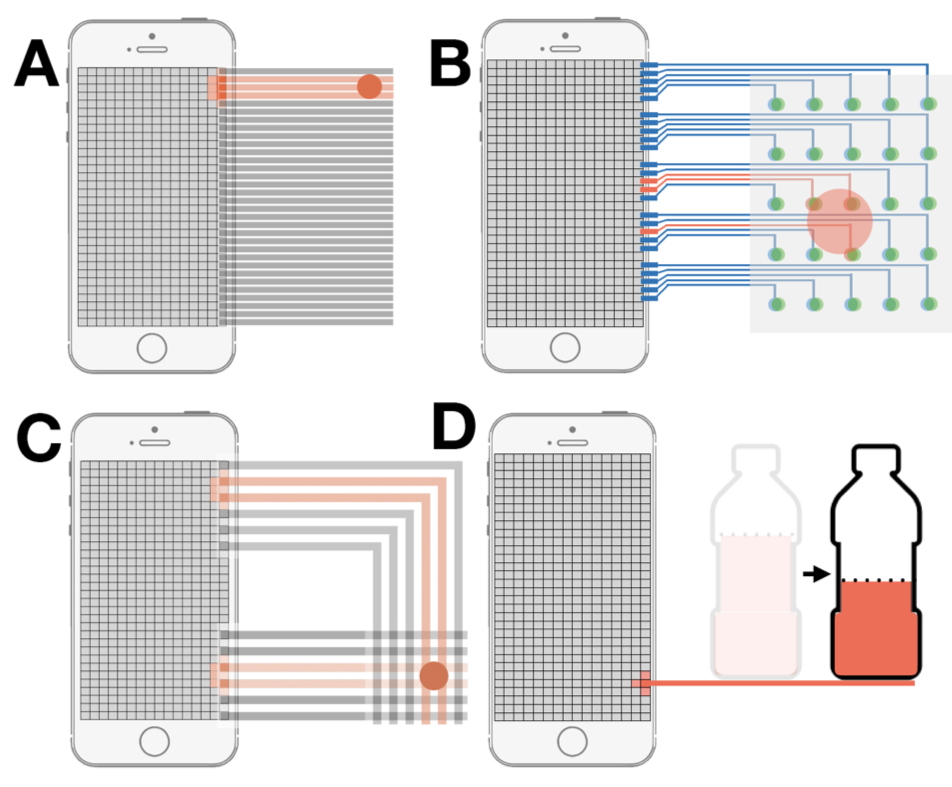
\includegraphics[width=0.95\columnwidth]{figures/1d2d-principle.png}
  \caption{\textit{FlexTouch} supports various applications with different sensing capabilities including A: 1D touch sensing, B:2D continuous multi-touch tracking, C: 2D High resolution single touch tracking and D: Object presence and state sensing}
  \label{fig:1d2d-principle}
\end{figure}

\section{Signal Processing for Touch Event Detection}
In this section, we use the P20 phone as an example to present the signal processing and the touch event detection pipeline of \textit{FlexTouch}. 

Fig ~\ref{fig:processing} demonstrates the signal processing procedure to detect the touch event on a 3-meter extension tape attached to the touchscreen. To filter out the high-frequency background noises, we applied a moving-average filter on the raw capacitive data using the unweighted mean of the previous 10 data points. During a touch event, a sharp signal rise occurs. To detect these rising step events, we applied a sliding window that contains 20 data points on a low-pass filtered signal. The step event can be extracted by comparing the data samples in front of the sliding window queue and at the tail of the queue. Each data sample in the black line graph in Fig ~\ref{fig:processing} is calculated using the following equation where $S_{i}$ represents the filtered capacitive data. 

\begin{equation}
    S_{diff} = \frac{S_{16} + S_{17} + S_{18} + S_{19}}{4}  - \frac{S_{0} + S_{1} + S_{2} + S_{3}}{4}
\end{equation}

Here we define the \textbf{\textit{signal-to-noise ratio (SNR)}} representing the signal strength of the raw capacitive data. As shown in Fig ~\ref{fig:processing}, we define the \textbf{\textit{Noise}} to be the difference between the maximum and minimum values of 100 data points for P20 before the touch event. The \textbf{\textit{Signal}} is the $S_{diff}$. To extract the touch signal from the background noise effectively, the SNR should be greater than a predetermined threshold. In theory, if SNR > 1, we can detect touch events. 

\begin{figure}[ht]
    \centering
      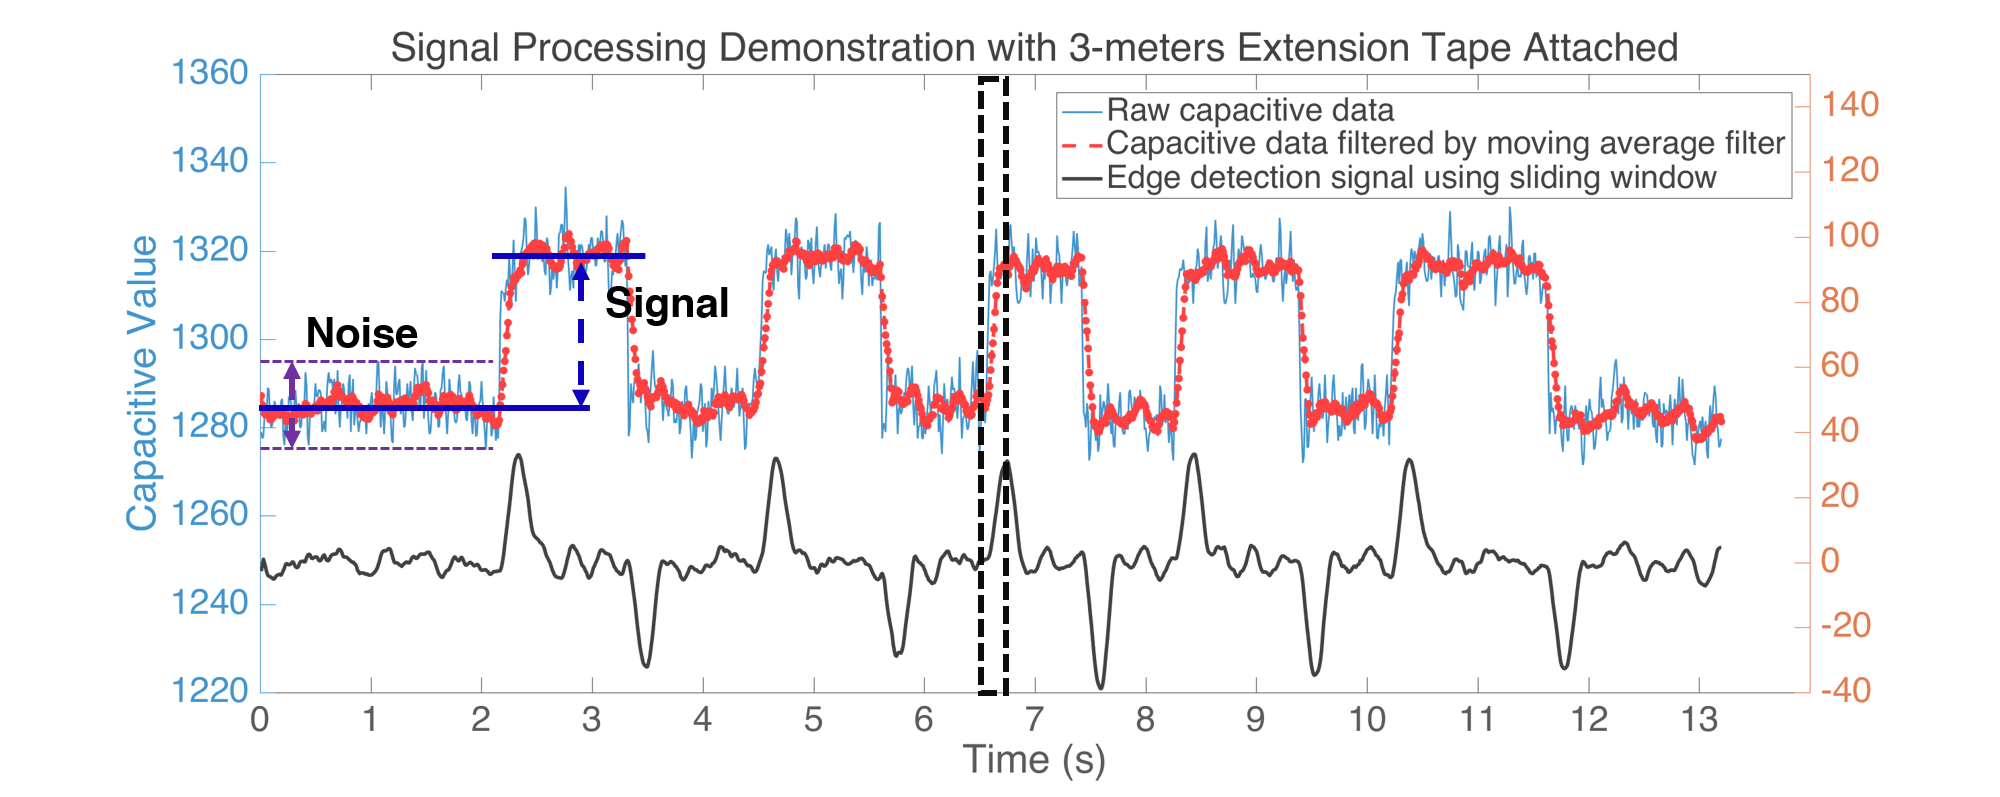
\includegraphics[width=0.95\columnwidth]{figures/processing.png}
      \setlength{\belowcaptionskip}{-8pt}
      \caption{Signal processing demo  detecting the touch event.}
      \label{fig:processing}
\end{figure}

\section{Differentiation Between On-screen and Off-screen Event}
% to be added tomorrow
% one figure 

\section{Fabrication}
We identified materials that can be easily customized into everyday surfaces with properties including flexibility, conductivity, and commercial availability. We fabricated interfaces using these materials through various processes, including adhering, cutting (e.g., manual cutting, laser cutting) and coating methods (e.g., ink-jet printing, brush painting). We leveraged the following materials to fabricate \textit{FlexTouch} interfaces.

\subsection{Conductive Tapes}
Conductive adhesive tapes are widely used for electromagnetic shielding and transmission wiring (e.g. paper circuits). The most widely available conductive tape is an adhesive copper foil tape that can be found at most hardware, electronic or gardening stores (Fig ~\ref{fig:material} A). It is \$2.50 per roll (6.3 mm x 20 m). The copper tape is highly conductive on both sides (0.05 $\Omega$ per square centimeter).

End-users can manually arrange any layout on any surface using copper foil tapes (e.g., Fig ~\ref{fig:material} E) without any additional fabrication equipment. In addition, the conductive tape is more flexible and suitable for large-scale applications since it can easily adhere to everyday objects. However, the copper foil tape is not suitable for volume production since it is not compatible with current fabricating techniques such as laser cutting or printing.

\begin{figure}
\centering
  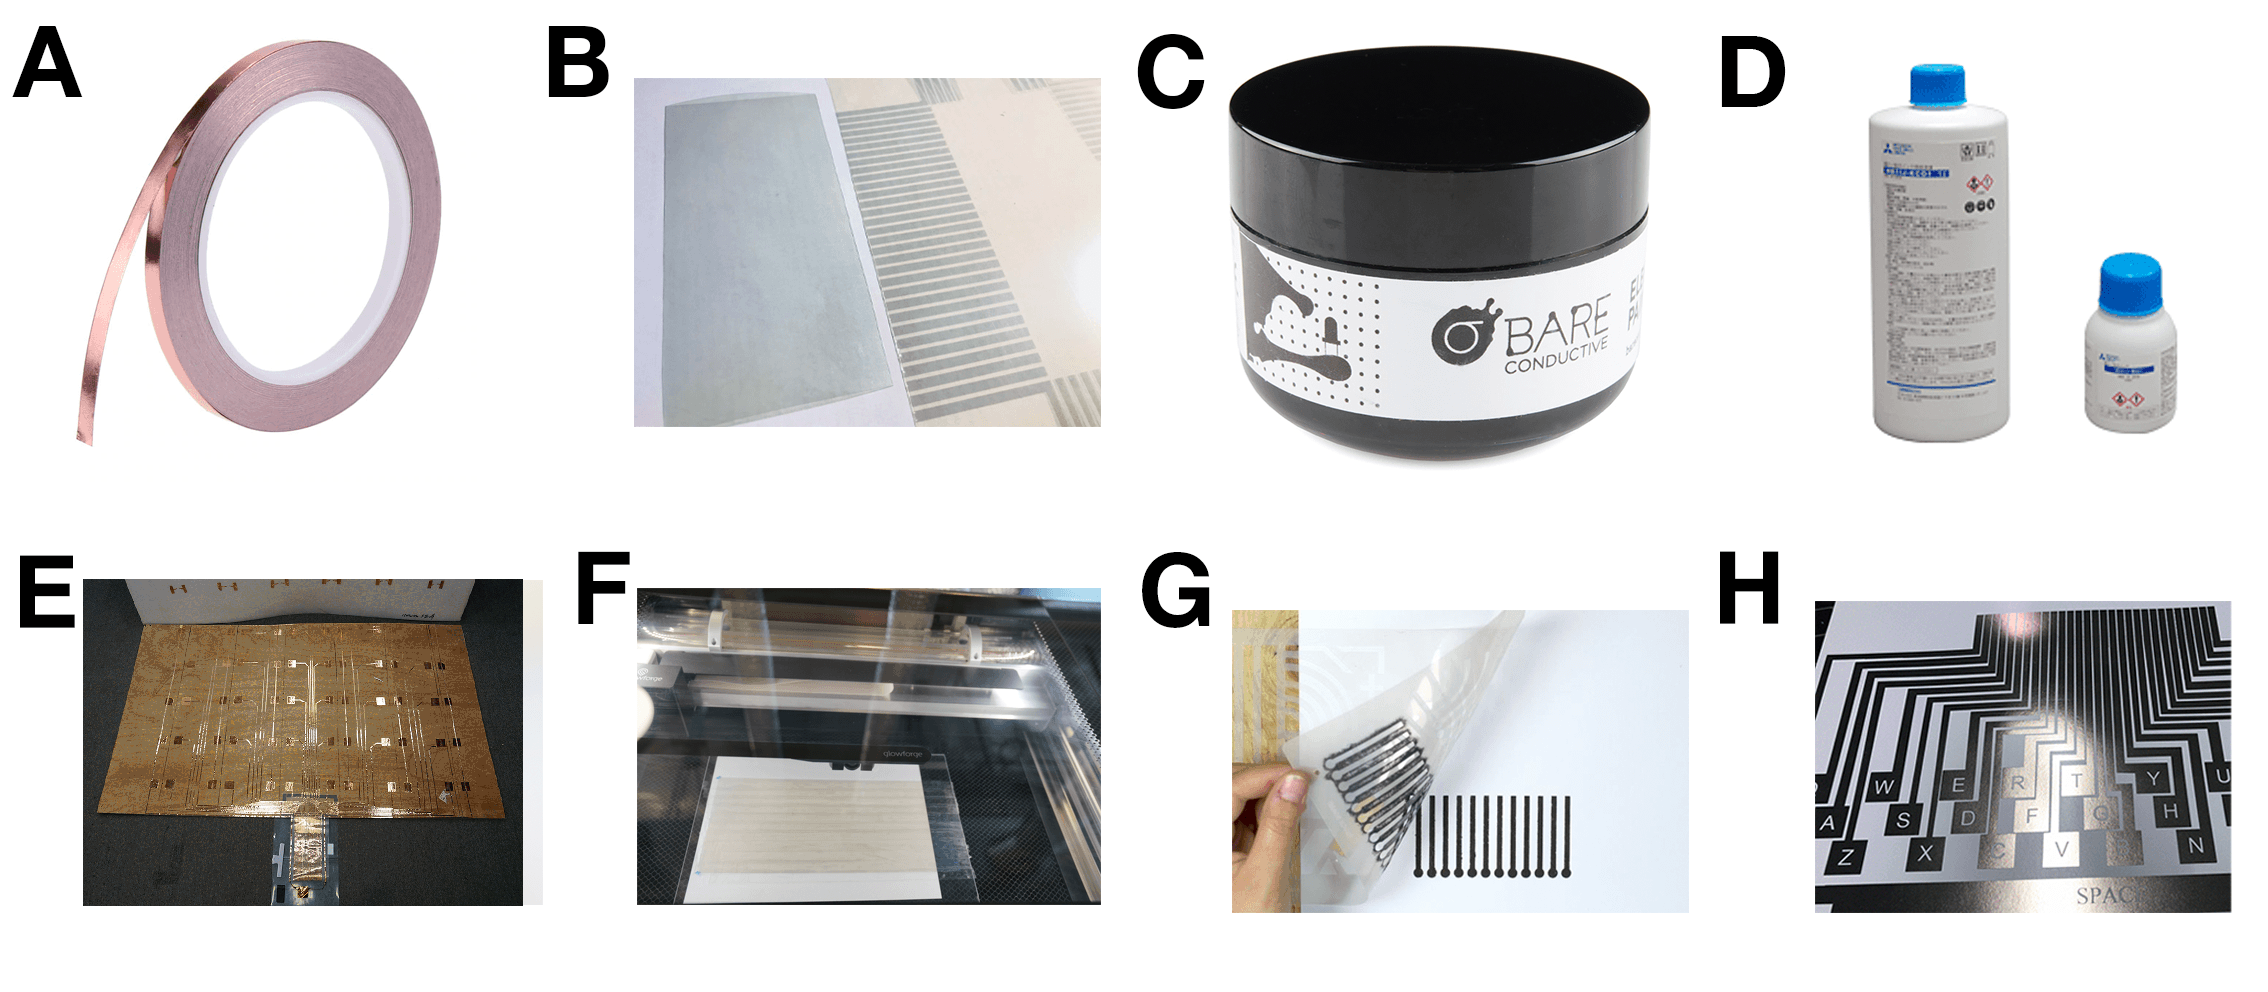
\includegraphics[width=0.95\columnwidth]{figures/material.png}
  \setlength{\belowcaptionskip}{-6pt}
  \caption{Commercially available materials. Copper foil tape (A) can be fixed to any surface (E). ITO PET Plastic film (B) can be fabricated to any 2D pattern using a laser cutter (F) or manually. Bare conductive carbon paint (C) and screen painting (G). Ink-jet circuit printer with Mitsubishi Silver nanoparticle ink (D) for printable conductive 2D layout (H). }
  \label{fig:material}
\end{figure}

\subsection{Conductive Films}
Film-like materials can be subtracted to 2D patterns using cutting or etching fabrication methods. One example material is the flexible Indium Tin Oxide (ITO) coated PET plastic film that is semi-transparent and conductive. We use the commercially available ITO-coated PET film manufactured by HNXCKJ ~\cite{ITO} that is compatible with laser cutters. Furthermore, 2D custom layouts are also available by coating ITO materials on extremely thin ($0.05 mm$) plastic film at a cost of \$30 per square foot (Fig ~\ref{fig:material} B).

Since the ITO-coated PET plastic film is highly transparent, it can be attached to the touchscreen without occluding the display (Fig ~\ref{fig:plugandplay} A). The ITO film can be customized as a screen protector for daily use with an array of ITO strips attached to the edges of the screen. This ITO strip array interface can be connected to the external application easily with a plug and play design as Fig \ref{fig:plugandplay} A and B show.

\subsection{Conductive Coating}
Liquid paint coating and ink printing are more versatile, as they can be added onto any surface in post-production. We identified two coating materials as examples. We use conductive carbon paint from Bare Conductive (Fig ~\ref{fig:material} C, \$280 per litter).  This material can be painted on a flat surface such as a wooden board or cardboard, and then laser cut to engrave the layout on top of it. Another suitable coating material is printable ink. We identified Silver nanoparticle ink made by Mitsubishi (Fig ~\ref{fig:material} D, \$340 per 100 ML) as presented by Instant Inkjet Circuits ~\cite{Kawahara-inkjet}. We fabricated the inkjet printable circuit with a Brother MFC-J480DW model printer. 

The conductive coating method is compatible with mass production due to its reproducibility. However, because of the limited size of each template or substrate, we need to further assemble the fabricated elements for large-scale application.

\section{Plug and Play}
In this section, we present \textit{FlexTouch}'s plug and play interface for daily use by proposing two assembly approaches as demonstrated in Fig ~\ref{fig:plugandplay}. 

\begin{figure}[ht]
    \centering
      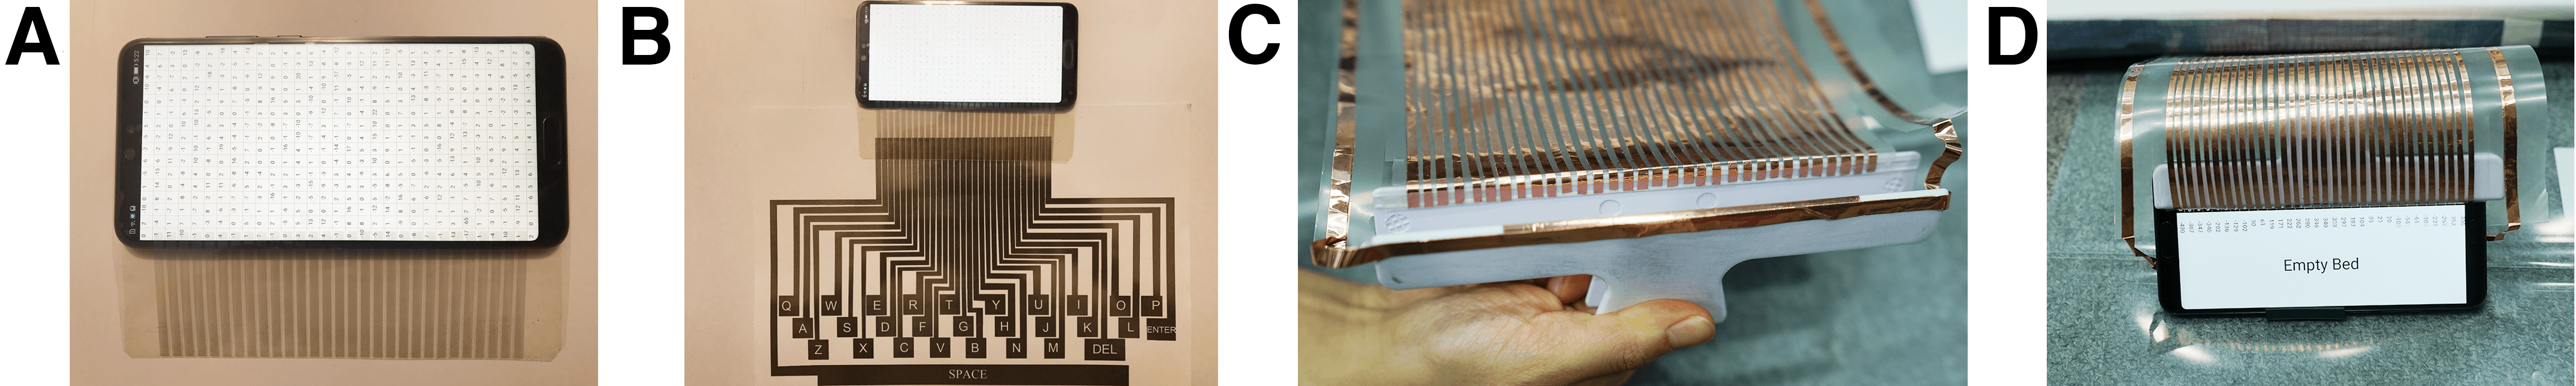
\includegraphics[width=0.75\columnwidth]{figures/plugandplay.png}
      \setlength{\belowcaptionskip}{-6pt}
      \caption{Demonstration of two assembly methods. The ITO strip array interface (A) can be stuck to a 2D-patterned application (B). The external application can be clipped onto the edge of the touchscreen (C and D).}
      \label{fig:plugandplay}
\end{figure}

\begin{itemize}
    \item \textbf{Adhere the external application with an ITO array film.} The ITO film is suitable for being integrated into a screen protector with an ITO conductive array connected to the edge of the touchscreen. The adhesive ITO film can easily be attached or detached to the external 2D patterned application. 
    \item \textbf{Fix the external application on the phone's edge with a clip.} The external application is connected with an array of conductive threads on one side of the clip while the electrodes on the 2D pattern representing the local ground are connected on the other side of the clip as shown in Fig ~\ref{fig:plugandplay} C. The customized part can be clipped onto the edge of the touchscreen as shown in Fig ~\ref{fig:plugandplay} D. 
\end{itemize}




\chapter{FlexTouch Sensing Capability Evaluation}
In this section, we evaluate the sensing range of \textit{FlexTouch} considering the effects of several factors including fabrication materials, the signal strip's dimension, sensing hardware and the configuration of the grounding strip.

\section{Evaluating Sensing Range with Variable Fabrication Material, Hardware, and the Local Ground}

Fig ~\ref{fig:experiment} illustrates our hardware setup for this study. Two strips are coming out from the phone. The signal strip is directly attached to the phone touch surface by a plastic clamp, while the grounding strip is connected to the back plate of the phone. In this study, we only look at the difference between using and not using the grounding strip. We discuss other variables pertaining to the  grounding strip in a more thorough study in later parts of this section. 

\begin{figure}[ht]
	\centering
	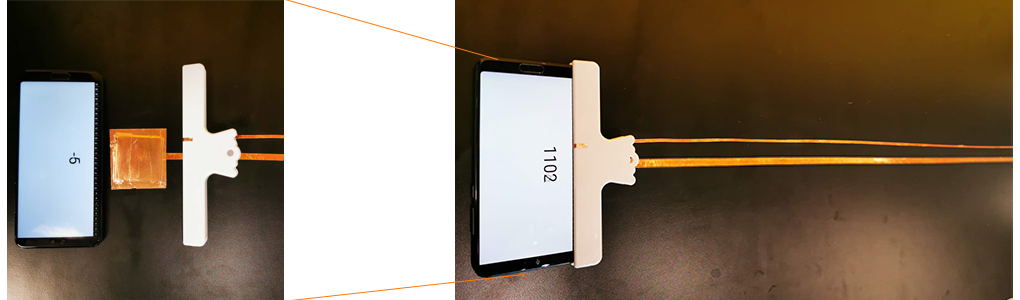
\includegraphics[width=0.70\columnwidth]{figures/evaluation_env.png}
	\setlength{\belowcaptionskip}{-6pt}
    \caption{Experiment setup to evaluate the touch sensing coverage range.}
    \label{fig:experiment}
\end{figure}
	
To evaluate the effect of different materials, We fabricated four different 5-meter long signal strips using materials including copper foil tape (CFT), ITO PET film (IPF), carbon paint (CP), and silver nanoparticle ink (SNI) with a fixed width of $1.5mm$. We set the grounding strip (5-meter long, $6mm$-wide copper foil tape) $2 cm$ away from the signal strip in this study. We recruited four participants for this experiment with an average age of 26.5 ($SD = 2.5$). The study lasted for 2 hours in total and we compensated each participant with a \$50 dollar gift card.

1) We attached the signal strip to the central position of the 8th sensing node on the touchscreen's left edge at the beginning of each session. In each session, we randomly selected two participants to perform a one-second finger touch on the far end of the signal strip five times followed by a one-second finger touch on the far end of both the signal and the grounding strips (also five times). Then we attached the signal strip to the 18th sensing node and repeat above procedure. 

2) We switched the phone hardware and repeated step 1).

3) We cut both signal and grounding strips to the next neighboring length following the order of 5m, 4m, 3m, 2.5m, 2m, 1.5m, 1m, 0.5m, 0.25m and 0.1m in sequence and repeated steps 1) and 2).

4) After completing the test on one material, we replaced it with another signal strip made of different material and repeated the experiment. Participants took a two-minute break between material switches.


\begin{table}[ht]
\caption{Average SNR versus extension distance under different configurations. (CFT: copper foil tap, IPF: ITO PET film, CP: carbon paint, SNI: silver nanoparticle ink)}
\vspace{-2mm}
\centering
	\begin{tabular}{|c|c|c|c|c|c|c|c|c|c|c|}
	
	\hline
	\textbf{Length[m]} & \textbf{0.10} & \textbf{0.25} & \textbf{0.50} & \textbf{1.00} & \textbf{1.50} & \textbf{2.00} & \textbf{2.50} & \textbf{3.00} & \textbf{4.00} & \textbf{5.00} \\
	\hline
	P20, CFT & 6.8 & 3.5 & 1.6 & 1.1 & 0.6 & - & - & - & - & - \\\hline
    P20, IPF & 6.6 & 3.4 & 1.4 & 0.9 & 0.5 & - & - & - & - & -  \\\hline
	P20, CP &  6.5 & 3.1 & 1.9 & 0.8 & - & - & - & - & - & -  \\\hline
	P20, SNI & 6.4 & 2.9 & 1.3 & 0.9 & - & - & - & - & - & -  \\\hline
	P20, CFT w/ GND &  15.8 & 9.8 & 5.8 & 4.7 & 3.3 & 2.6 & 2.0 & 1.5 & 1.3 & 0.7 \\\hline
	P20, IPF w/ GND &  16.5 & 10.8 & 5.5 & 4.0 & 3.1 & 2.0 & 1.6 & 1.1 & 0.8 & 0.5 \\\hline
	P20, CP w/ GND & 15.4 & 10.1 & 6.0 & 3.7 & 2.2 & 1.7 & 1.0 & 0.8 & - & - \\\hline
	P20, SNI w/ GND & 15.3 & 9.8 & 5.4 & 3.1 & 2.2 & 1.7 & 1.4 & 1.2 & 0.9 & 0.5  \\\hline

	P10, CFT & 15.7 & 7.6 & 4.3 & 2.7 & 1.7 & 1.1 & 0.7 & - & - & - \\\hline
	P10, IPF  & 14.2 & 7.5 & 3.9 & 2.9 & 1.4 & 1.0 & 0.5 & - & - & - \\\hline
	P10, CP &  14.4 & 6.8 & 3.2 & 1.6 & 0.8 & 0.5 & - & - & - & - \\\hline
	P10, SNI & 14.9 & 6.9 & 3.1 & 2.8 & 1.4 & 1.0 & 0.6 & - & - & -  \\\hline
	P10, CFT w/ GND & 20.4 & 10.2 & 7.0 & 4.3 & 3.1 & 2.3 & 1.9 & 1.5 & 1.1 & 0.8 \\\hline
	P10, IPF w/ GND  &  21.4 & 11.5 & 7.9 & 5.3 & 3.2 & 2.7 & 1.7 & 1.2 & 0.8 & 0.5 \\\hline
	P10, CP w/ GND & 20.1 & 12.4 & 8.1 & 4.3 & 2.8 & 2.1 & 1.2 & 0.7 & - & - \\\hline
	P10, SNI w/ GND &  19.4 & 11.2 & 8.6 & 4.1 & 2.8 & 2.0 & 1.6 & 1.2 & 0.8 & 0.5 \\\hline
	\end{tabular}
	
	\label{tab:snrtable}
	
\end{table}

\subsection{Results}

We summarize our results in Table ~\ref{tab:snrtable}, which outlines the signal strength illustrated by the SNR value of our system. There are a total of 16 different hardware/material/grounding strip's presence configurations and each of them has ten different signal strip length configurations. We highlight the following insights gained from this evaluation study:

\textbf{1. \textit{FlexTouch} can support large-scale capacitive sensing applications with a coverage range of up to 4 meters.}  Using the  threshold of SNR > 1, we observe that the minimum sensing distance supported by \textit{FlexTouch} exceeded 0.5 meters regardless of the hardware, the material, and the grounding strip's presence. However, the grounding strip helps extend the sensing range significantly: Under the best conditions, with both the p10 and p20 hardware and CFT material, \textit{Flextouch} could reach coverage distance of more than 4 meters.

\textbf{2. \textit{FlexTouch}'s sensing range is positively correlated with material conductivity.} Among the four materials, CFT achieved the longest sensing range, following by SNI and IPF, finally by CP. This ordering is consistent with the conductivity ordering of the 4 materials presented in Figure ~\ref{fig:material-width} B. We believe that materials with even better conductivity may be able to exceed the sensing range we observed in this study. 

\begin{figure}[ht]  
\centering
  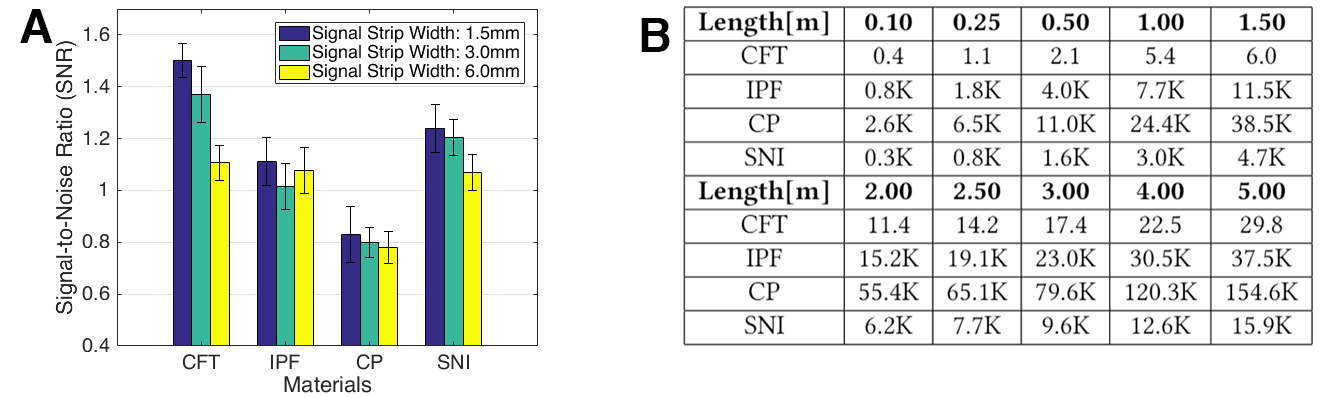
\includegraphics[width=0.75\columnwidth]{figures/material-width-and-table.png}

  \setlength{\belowcaptionskip}{-8pt}
  \caption{The SNR versus the signal strip width using four different materials (A). The table of material's resistance values ($\Omega$) under different extension lengths (B).}
  \label{fig:material-width}
\end{figure}

\textbf{3. The extension distance increases as the width of the signal strip decreases.} To better understand the effect of the width of the signal strip, we conducted a follow-up study changing the width of the signal strip made with 4 different materials with a fixed length of 3 meters. We recorded the SNR in Figure ~\ref{fig:material-width} A, which demonstrates that \textit{FlexTouch} has the best performance with a $1.5mm$-wide signal strip regardless of the fabrication material. We believe that even thinner strip will be able to support longer sensing ranges. However, since a thinner strip is less conductive, we believe that there's a lower limit on the strip's width.


\textbf{4. \textbf{\textit{FlexTouch}} can not differentiate touchpoints at different locations on the extension strip with the presence of the ground plane.} We evaluated the touch resolution on a single pair of extension strips by touching on different positions with a $50 cm$-step using different materials. We did not observe that 2D touch input could be enabled with single-layer conductive materials as prior work ~\cite{Ikematsu-Ohmic-Touch, mobicom-gao18} mentioned with the grounding strip's presence.

\textbf{5. No significant difference in using different capacitive sensing hardware}. The 2 different phones being employed in our study, Huawei p10 and P20 demonstrate moderate SNR difference when the same material is being deployed with a length below $1m$. However, when the strip length continued to increase, the SNR demonstrated similar results when all other variables are consistent. Given limited hardware resources, we were only able to evaluate these two phone models. Future studies that include capacitive touchscreens from different manufacturers will be necessary to fully understand the impact of capacitive touchscreens on the feasible sensing range of our system.

\subsection{Study Results in Relation to the Proposed Working Principle}
 
Results in Table ~\ref{tab:snrtable} show that as the length of the sensing strip increases linearly, the touch signal strength decreases logarithmically. As presented in section \textit{FlexTouch: Working Principles}, the finger touch introduces additional shunt circuit changing $C_{e}$ to $C_{eg}$. We assume the values of $C_{f}$, $C_{m}$, $C_{p}$ are 5 pF, 10 pF and 10 pF while $C_{eg} = 1.5 \times C_{e}$. Then Formula (2) can be presented as following.

Before the touch event:
\begin{equation}
    \tau_{b} = a\frac{100 + 10C_{e}}{20+C_{e}}
\end{equation}

After the finger touch on the signal strip only as well as on both the signal strip and the grounding strip: 
\begin{equation}
    \tau_{af} = a\frac{150 + 10C_{e}}{25+C_{e}}, \tau_{ag} = a\frac{150 + 15C_{e}}{25+1.5C_{e}}
\end{equation}

The estimated capacitance value can be represented as:
\begin{equation}
    \tau_{df} = \tau_{af} - \tau_{b},  \tau_{dg} = \tau_{ag} - \tau_{b}
\end{equation}

We assume that $C_{e} = 100 \times L$ where $L$ represents the length (meter) of the strip since the width is assumed to be static. The curve of how the estimated capacitive value along the strip length matches the measured raw data if $a$ is assigned to 600. The pattern we see in our result matches with the model we built for explaining \textit{FlexTouch}'s working principle. 

\section{Understanding the Effect of the Grounding Strip}
The previous study shows the significant effect of introducing the grounding strip into the extension circuit design. There are additional variables such as the distance between the grounding strip and the signal strip, the width of the grounding strip as well as the material of the grounding strip that we would like to further evaluate to provide in-depth insights into designing touch sensing solutions with \textit{FlexTouch} in this section.

\subsection{Effect of the Gap Between Grounding and Signal Strips}

We used copper foil tape as example material to examine the effect of the gap between the grounding strip and the signal strip on the maximum touch sensing distance. We set the grounding strip's width to be $6 mm$. We measured the maximum coverage with the following variables. 1) Gap distance between the central lines between the signal and grounding strips: $0.5 cm$,  $1 cm$, $2 cm$, $3 cm$, $5 cm$ and $10 cm$. 2) Signal strip's width: $1.5 mm$ and $3.0 mm$. 3) Touch postures: single index finger touch and dual index finger touch with two hands.

To measure the maximum touch sensing distance, we started with the maximum sensing distance measured in the previous study. In each session, we increased/decreased the extension distance by sticking/cutting additional $n$ pieces of $10 cm$-long copper foil tape at the far ends of both the grounding and signal strips. We recruited four participants for this study with an average age of 25.5 (SD = 1.5). They performed three touches with each touch posture at the far ends the extension strips. We repeated the above sessions until the SNR exceeded 1.0 for both single-finger and double-finger touches. We repeated the above procedure five times to obtain an average coverage distance for each condition. 

\textbf{1. The maximum touch sensing distance increases logarithmically as the gap distance between the grounding strip and signal strip increases.} As shown in Figure \ref{fig:ground-effect}, there exists an upper limit on the touching sensing coverage distance around 5 meters regarding the gap distance and the signal strip's width. However, although larger gap distance results in better sensing coverage distance, it limits the number of strips that can be deployed for any given space.

\textbf{2. Touch posture has no significant effect on the coverage distance performance.} There is no significant difference between touches with one finger or two fingers from two hands ($F_{1,89} = 0.32, p = 0.54$). We envision that future work could connect the local ground directly to users and not to the extension circuit, enabling longer sensing range and higher resolution design.


\begin{figure}[ht]
\centering
  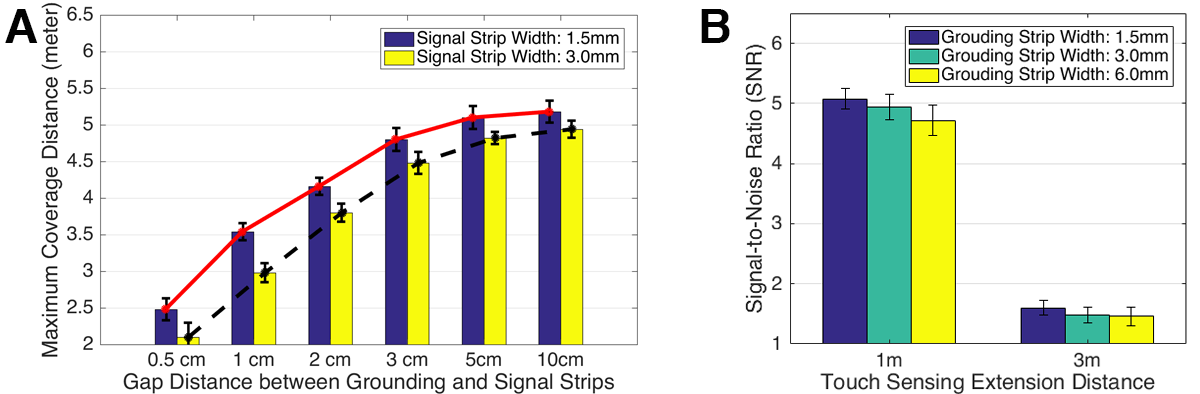
\includegraphics[width=0.7\columnwidth]{figures/grouding-gap-and-width.png}
  \setlength{\belowcaptionskip}{-8pt}
  \caption{Maximum touch sensing distance versus the gap distance between signal and grounding strips (A). SNR versus the grounding strip width with different extension distances (B).}~\label{fig:ground-effect}
\end{figure}

\subsection{Effect of Grounding Strip Width}

We used copper foil tape as example material to examine the effect of the grounding strip width on the touch sensing distance. We set the gap distance between extension strips to be $2 cm$ and the signal strip width to be $1.5 mm$. We measured the signal strength on fixed extension distances ($1m$ and $3m$) with different grounding strip's width: $1.5 mm$, $3.0 mm$ and $6 mm$. We recruited four users to touch the far ends of the paired extension strips three times for each condition. We repeated the above procedure five times to obtain an average measured SNR. We highlight the following insights gained from this evaluation study:


\textbf{The touch sensing coverage distance is negatively correlated with the grounding strip's width.} We recorded the SNR values in Figure \ref{fig:ground-effect} B, which demonstrates that \textit{FlexTouch} has the best performance with the $1.5mm$-wide signal strip. We recommend a thinner signal strip that can support better sensing range performance as well as higher resolution design. Combined with the result on the signal strip's width in Section $5.1.1$, we believe that the sensing distance can be further extended if we adopt $1.5 mm$-wide or thinner copper foil tape for both the signal and grounding strips.

\subsection{Effect of the Grounding Strip Material}
In this study, we explored whether grounding strip material affects the sensing distance performance. We set the signal strip material to be copper foil tape, the gap distance between extension strips to be $2 cm$ and the widths of both the signal strip and grounding strip to be $6.0 mm$. We measured the SNR values of 1-meter and 3-meters sensing distance with four different grounding strip's materials. The result is illustrated in Table \ref{tab:gnd-material}.

\begin{table}[ht]
\caption{Average (standard deviation) SNR values with one strip made of CFT and the other made of one of the three materials.}
\vspace{-2mm}
\centering
	\begin{tabular}{|c|c|c|c|c|c|c|c|}
	\hline
	Material &\textbf{CFT} & \multicolumn{2}{c|}{\textbf{IPF}} & \multicolumn{2}{c|}{\textbf{CP}} & \multicolumn{2}{c|}{\textbf{SNI}} \\
	\hline
    Condition & \textbf{reference} & \textbf{ground} & \textbf{signal} & \textbf{ground} & \textbf{signal} & \textbf{ground} & \textbf{signal}  \\
	\hline
	
	$1m$ sensing distance & 1.14 (0.07) & 1.06 (0.11) & 1.07 (0.13) & 0.88 (0.12) & 0.86 (0.10) & 1.11 (0.14) & 1.09 (0.13) \\
	\hline
	$3m$ sensing distance & 3.40 (0.20) & 3.31 (0.25) & 3.35 (0.23) & 3.22 (0.12) & 3.20 (0.08) & 3.42 (0.13) & 3.37 (0.14)   \\
	\hline
	\end{tabular}
	\label{tab:gnd-material}
	
\end{table}

\textbf{1. \textit{FlexTouch} sensing range is positively correlated with material conductivity of the \textit{grounding strip} in general.} Similar to the results in Section \textit{5.1.1}, we found that the material conductivity has a positive effect on the sensing range performance.

Then we switched the grounding strip and the signal strip which are made of different materials and noticed that:
 
\textbf{2. Signal strip and ground strip made of different materials are interchangeable when they have the same width.} We found no significant difference in the signal strength when switched the two strips with the same width but different materials. 

\subsection{Study Results in Relation to the Proposed Working Principle }
Section $5.1.2$ explains the relationship between signal strength and the extension strip's length using the working principle hypotheses in Section $3$. We explain the results we found in study 2 that pertain to the effect of separation - $d$ as well as fabrication material - $\varepsilon$.

To enhance the effect introduced by touch, less capacitance between the signal strip and the grounding strip is preferred, which is represented as $C_{e}$. The sensing distance can be represented as: 

\begin{equation}
    L = \frac{C_{e} \times d}{\varepsilon \times D}
\end{equation}

Therefore, we conclude that smaller extension strip width ($D$), larger gap distance ($d$), more conductive material and more insulating material between strips (smaller $\varepsilon$) will help extend the sensing range, which is consistent with our study's results.

\section{Evaluating Object Presence Sensing Capabilities}
Given the capacitive nature of \textit{FlexTouch}'s sensing principle, it can go beyond sensing touch events. Everyday objects that contain capacitance also draw electric current from the touchscreen and can be detected by \textit{FlexTouch}. In this section, we evaluate the feasibility of detecting everyday objects' presence using \textit{FlexTouch}. 

\subsection{Apparatus and Procedure}
In this study, we used $3.0 mm$ wide copper foil tape and a Huawei P20 phone. We explored a range of factors that may affect \textit{FlexTouch}'s capability in sensing everyday objects' presence: the dielectric property and materials of different everyday objects, the length of the extension strips as well as the presence of the local ground. We used the following procedure in the experiment:

1) We attached the signal strip to the central position of the 19th sensing node on the left edge of the touchscreen. Then we started the testing application on the phone sending the raw capacitive data to a local server running on a laptop for later analysis.

2) We placed 11 pre-selected objects in random order at the end of the signal strip without the grounding strip's presence for around 2 seconds then on both the signal and grounding strips for another 2 seconds. We picked up and re-placed the object five times, ensuring the object was in contact with the strips on each placement.

3) We trimmed the strips in order of the following lengths: 3m, 2m, 1.5m, 1m, 0.5m, 0.25m, 0.1m and repeated step 2).

\subsection{Results}

Table ~\ref{tab:snrtableforobj} presents the average SNR value with 22 configurations across everyday objects and the presence of the grounding strip.

As presented in Table ~\ref{tab:snrtableforobj}, \textit{FlexTouch} can sense the presence of everyday objects by detecting the current they draw via the extension strip. The second column in Table ~\ref{tab:snrtableforobj} illustrates that all the objects change the capacitive signal extended from the touchscreen on the phone. However, the sensing range varies with the object's material. Objects made of metal have the strongest signal strength. The coverage distance ranges from $50 cm$ to $2 m$. Besides, pairing the local ground with the touch screen extension strip can dramatically enhance the object detection's sensing range. 

\begin{table}[ht]
\caption{Average SNRs versus extension strips' lengths with different everyday objects. The table's X and  Y values (X/Y) represents the SNR values of conditions with and without the grounding strip. }
\vspace{-2mm}
	\centering
		\begin{tabular}{|c|c|c|c|c|c|c|c|c|}
		\hline
		\textbf{Length[m]} & \textbf{0.10} & \textbf{0.25} & \textbf{0.50} & \textbf{1.00} & \textbf{1.50} & \textbf{2.00} & \textbf{3.00} \\
		\hline
		Finger Touch (\textbf{reference}) & 15.8/6.8 & 9.8/3.5 & 5.8/1.6 & 4.7/1.1 & 3.3/0.6 & 2.6/- & 1.5/-  \\\hline
		$5 cm\times 5 cm$ Copper Foil Tape & 15.3/3.2 & 9.5/1.9 & 5.5/0.8 & 4.6/- & 3.0/- & 2.3/- & 1.3/-  \\\hline
		Stainless Steel Water Cup &  12.6/3.4 & 10.0/2.0 & 4.3/1.1 & 2.0/- & 1.6/- & 1.5/- & 0.7/-  \\\hline
		MacBook Pro 13' &  5.4/2.4 & 3.7/1.7 & 1.2/0.6 & 0.6/- & -/- & -/- & -/- \\\hline
		Carving Knife  & 5.6/1.5 & 2.7/0.6 & 1.3/- & -/- & -/- & -/- & -/-  \\\hline
		iPhone XR  & 4.6/2.5 & 2.5/2.0 & 1.2/0.5 & 0.7/- & -/- & -/- & -/- \\\hline
		550 ml Bottled Water  &  4.3/2.8 & 2.8/1.2 & 0.6/- & -/- & -/- & -/- & -/- \\\hline
		50 ml Bottled Water  &  3.1/1.3 & 2.0/0.7 &  -/- & -/- & -/- & -/- & -/- \\\hline
		Glass Cup &  2.7/0.6 & 1.0/- & -/- & -/- & -/- & -/- & -/-  \\\hline
		Notebook & 0.9/0.8 & -/- & -/- & -/- & -/- & -/- & -/-   \\\hline
		Cardboard Box  & 0.5/0.6 & -/- & -/- & -/- & -/- & -/- & -/-  \\\hline
		Mouse & 0.5/0.5 & -/- & -/- & -/- & -/- & -/- & -/- \\\hline
		\end{tabular}
		
		\label{tab:snrtableforobj}
		
	\end{table}



\chapter{Example Applications}
In this section, we present four example applications to demonstrate the versatility of \textit{Flextouch}, including examples of body posture recognition, 2D large-scale continuous touch tracking as well as sensing the presence of everyday objects. These applications demonstrate the possibility of new interaction methods and the sensing potential of \emph{FlexTouch}.

\section{Smart Mattress for Sleep Monitoring}
As \textit{FlexTouch}'s sensing range can reach up to 4 meters, we can leverage this long-range capability to detect users' behaviors while they're in bed. This is achieved by fabricating a three-layer structure with $5 \times 6 = 30$ sensing notes as presented in Fig ~\ref{fig:smartmattress} A - C. Each sensing node on the top layer is formed with a signal and a grounding electrode (Fig ~\ref{fig:smartmattress} B). All electrode pairs are connected to electrodes on the bottom layer. We placed a mattress on a wooden board and affixed a copper-tape circuit (Fig ~\ref{fig:smartmattress} C) with its electrodes connected with the electrodes on the bottom layer of the mattress. We activated the application by plugging in the touchscreen phone using a clip with an array of copper foil tapes attached (Fig ~\ref{fig:smartmattress} E to I). The material cost of this application was 10 USD.

\begin{figure}[ht]
  \centering
    \includegraphics[width=0.85\columnwidth]{figures/FlexTouch-mattress.png}
    \setlength{\belowcaptionskip}{-6pt}
    \caption{The structure of the smart mattress (A - C), the classification confusion matrix (D)  and the five detected states (E - I) with corresponding scenarios and raw sensing data visualization}
    \label{fig:smartmattress}
  \end{figure}

\subsection{User Evaluation}
To evaluate the performance of the smart mattress, we recruited eight pairs of participants (10 males) with an average age of 25.6 (SD = 2.2) and an average height of 170 cm (SD = 5.3) who we compensated with a \$20 gift card for a 30-minute test. There was one practice session followed by three data collection sessions. For each session, the paired participants followed the instruction of \textit{single user sitting on the bed}, \textit{single user lying on the bed}, \textit{one user sitting and one user lying on the bed}, \textit{two users lying on the bed} in order. The paired participants repeated the above procedure in each session five times and kept each posture for approximately 4 seconds. We logged the raw capacitive data with a Huawei P20 phone and logged the procedure with a camera for labeling. 

\subsection{Result}
All samples were manually labeled according to the video. We picked frames out of the series of data for each state. The dataset contains 120 data samples per posture across participants and each data sample includes 30 raw capacitive data points. The dataset was randomly split into 2 subsets (96 training samples and 24 testing samples). We conducted 5-fold cross-validation using the LibSVM classifier and achieved an average accuracy of 91.2\% across 5 states. We believe that the low resolution causes low recognition when users are sitting on the mattress, as Fig ~\ref{fig:smartmattress} D indicates. We discuss this result and future design recommendations in the later discussion section.   

\subsection{Smart Yoga Mat for Fitness Posture Detection}
The sensing range of \textit{FlexTouch} allows us to enable large-scale sensing applications such as a yoga mat.  \textit{FlexTouch} can detect and classify different user poses based on their capacitive profiles when working out on the yoga mat. Leveraging this functionality, smart home applications can adjust the surrounding environment based on users' physical activities. For instance, it could adjust ambient light, temperature, and music according to the user's activity on the yoga mat. The materials we used to build the touch-sensitive yoga mat cost just 8 USD. 

\begin{figure}[ht]
\centering
  \includegraphics[width=0.95\columnwidth]{figures/FlexTouch-yoga-new.png}
  \caption{Recognizing user's posture on the yoga mat built by \textit{FlexTouch} with raw sensing image data}  \label{fig:yogamat}
\end{figure}

As shown in figure ~\ref{fig:yogamat}, we built a 2D-patterned matrix ($8\times11 = 88$ sensing nodes) on a regular yoga mat using ITO strips, which can classify five different yoga poses (lord of the dance pose, plank, high lunge variation, camel pose and lotus pose).

\subsection{User Evaluation}
User Evaluation. We recruited 12 participants (6 males, 6 females, average age 27.7 (SD = 3.4), average height 171.2 cm (SD = 9.8). Each participant received \$10 for participating in this study, which included 1 practice session followed by three data collection sessions. Before each data collection session, the five postures were randomized. Then the participant performed each posture five times with a duration of 3 seconds. We logged the raw capacitive data with a Huawei P20 phone and logged the procedure with a camera for ground truth labeling.

\subsection{Results}
All samples were manually labeled according to the video. We picked the middle frame out of the series of data when the pose was performed. The dataset contains 180 data samples in total and each data sample includes 32 frames of raw capacitive data. We performed 5-fold cross-validation on the dataset (144 training samples and 36 testing samples for each iteration) using the LightGBM classifier and achieved an average accuracy of 97.1\% across 6 classes (five body postures and no action).

\section{Fitness Tracking on Count of Repetition, Speed and Distance}
In this example, we demonstrate fitness tracking applications when deploying \textit{FlexTouch} on a treadmill, cycling machine, and chest-press machine as shown in Figure ~\ref{fig:fitness}. Even though some recent commercial fitness machines have the function of sharing data to personal mobile devices, many machines are not embedded with this function such as chest press machine, lat pull-down gym machine, etc. Since these machines have similar periodic patterns, we propose these applications to inspire future designs by identifying the position where the sensing node is placed to sense states, state-changing events, and state-changing speed. We designed a binary sensor using a pair of $1.5m$-long, $3 mm$-wide copper foil tapes. Since the update rate of the Huawei P20 phone is 100 fps, the button sensor can detect not only the binary touch event but also how fast it changes. By counting the touch event frequency, we can calculate the distance or speed. This allows users to track their fitness behavior across devices at home or in the gym by simply plugging their phones into a customized passive module. Based on the tracking data, the application can customize fitness plans for individuals. This design cost 0.3 USD.

\begin{figure}[ht]
\centering
  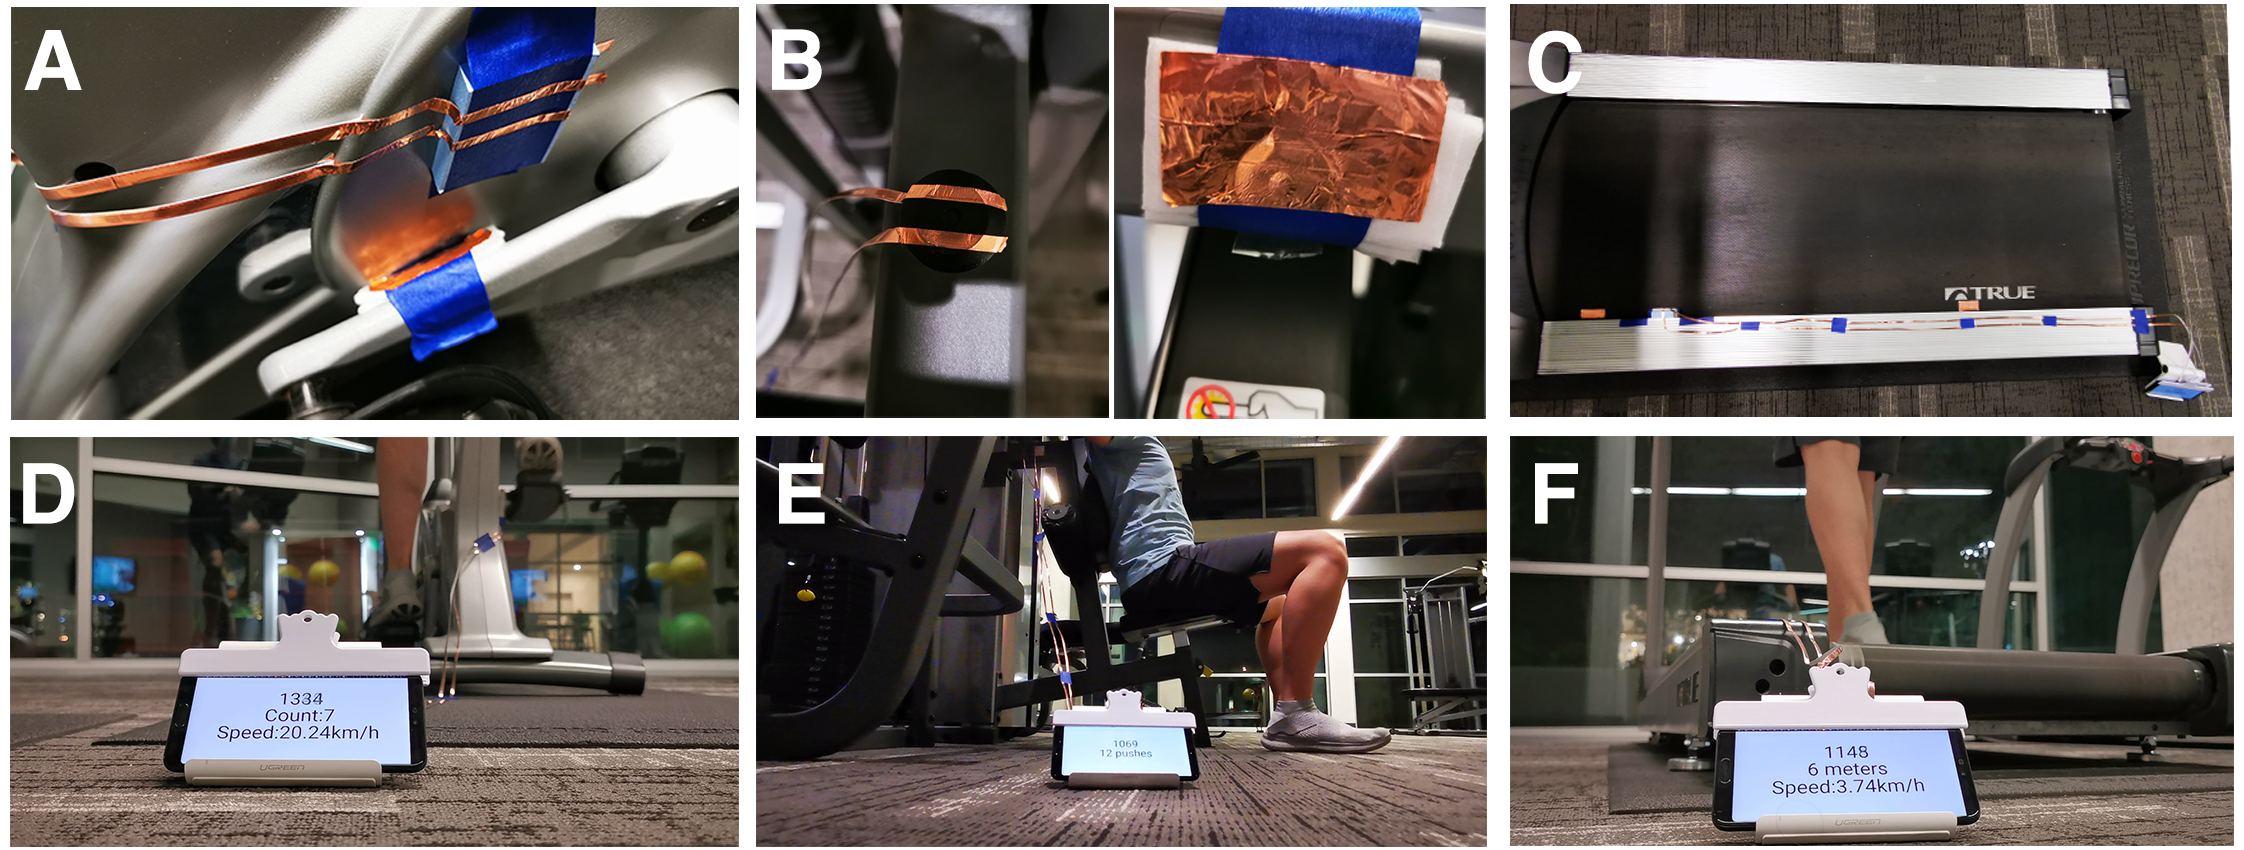
\includegraphics[width=0.7\columnwidth]{figures/gym.png}
  \setlength{\belowcaptionskip}{-4pt}
  \caption{Fitness tracking using \textit{FlexTouch}. A and D: speed tracking on a cycling machine. B and E: push counter on a chest-press machine. C and F: distance and speed tracking on a treadmill.}  
  \label{fig:fitness}
\end{figure}

\subsection{User Study}
To evaluate the tracking accuracy, we recruited six users (3 females, average age of 24.7 (SD = 0.8)). Each user finished three rounds of testing. For each round, users ran on the treadmill for 2 minutes with a maximum speed of $12KM/H$, rode the cycling machine for 2 minutes with a maximum speed of $25KM/H$, and, finally, finished the round with ten chest presses. The study lasted for 20 minutes and we compensated each participant with a \$20 dollar gift card. We used a camera attached on the display panel to record the speed and distance data from the fitness machine for ground truth annotation.

\subsection{Results}
We measured the maximum riding speed from the cycling machine, the maximum running speed and distance resolution from the treadmill as well as repeat counts from the chest-press machine. Since the signal processing algorithm stated in Section $4.4$ requires a minimum of 10 valid data to detect a touch event, there's an upper limit of the build button sensor's working frequency under 10 fps. Results indicate that \textit{FlexTouch} had an accuracy of 98.9\% on tracking the running and cycling speed and 100\% on tracking the chest-press count. Since the touch event happens once every cycle, our distance tracking resolution for the treadmill is 1.5 meter for the model that we tested.

\section{Smart Desk Reminder Application}
Given the flexible and passive nature of \textit{FlexTouch}, we recognize the potential to integrate it into large surfaces such as tables or desks to detect interaction with humans or everyday objects (Fig ~\ref{fig:smartdesk}). In this example, we placed three sensing nodes $40 cm$ away from the touchscreen to sense the user's body contact as well as one sensing node with $20 cm$ distance to sense the cup's water status (i.e. the amount of water remaining in the cup). When the user is working, instead of placing the phone on the desk, the user uses \textit{FlexTouch} to activate the smart desk application. It can remind users to take a break or stay hydrated by drinking water while they work continuously for a while. This is achieved by extending the touch sensing node to the desk where users lay their arm and place the water cup. The material cost for building this application was 0.30 USD.


\begin{figure}[ht]
\centering
  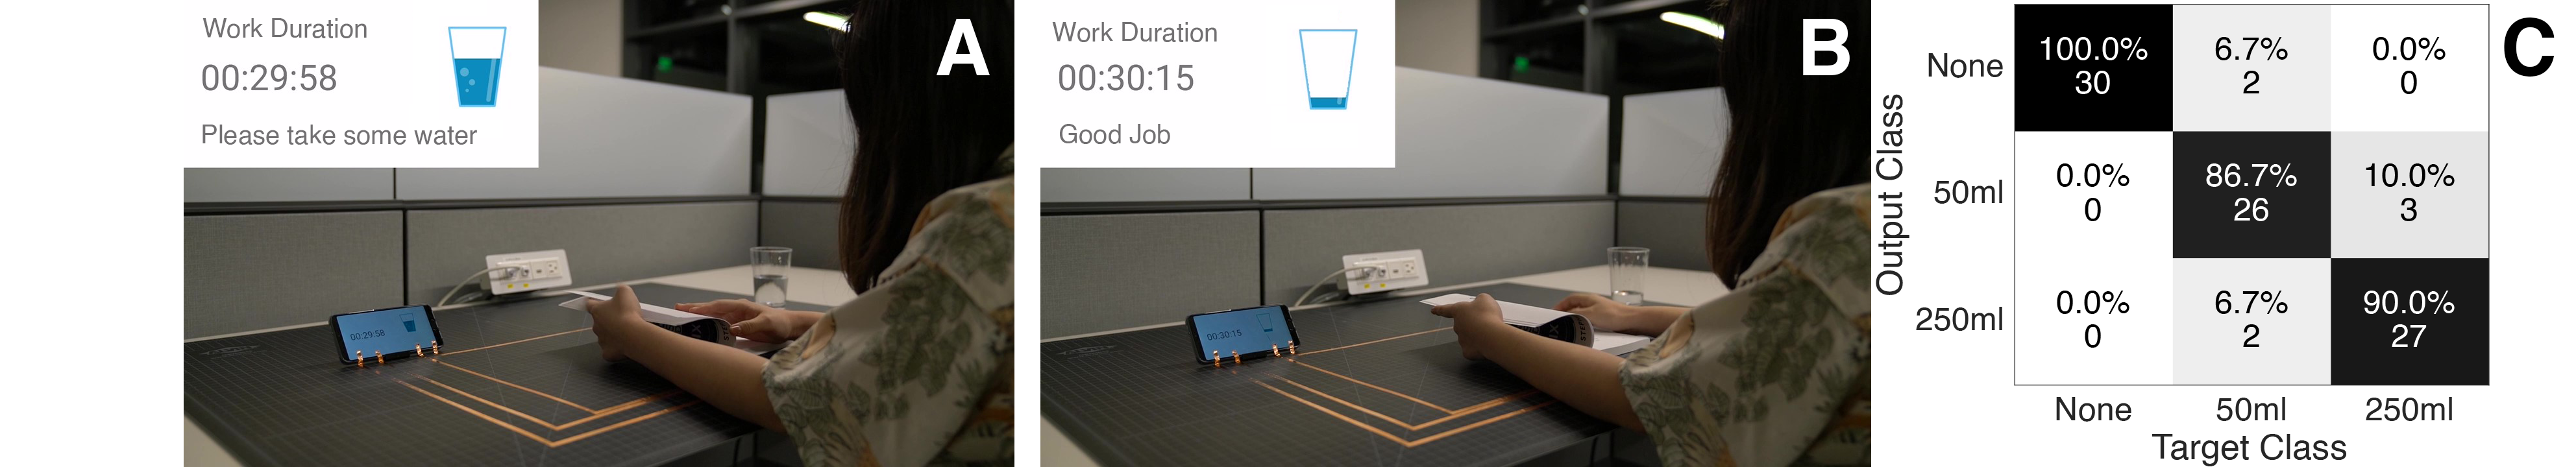
\includegraphics[width=0.8\columnwidth]{figures/FlexTouch-desk.png}
  \setlength{\belowcaptionskip}{-4pt}
  \caption{Smart desk example detecting user and object's presence and status}
  \label{fig:smartdesk}
\end{figure}

\subsection{User Study}
To evaluate the sensing performance on the presence and status of the user and the water cup, we conducted a user study in which six users (2 females, 4 males, average age of 25.0 (SD = 0.9)) participated. For each round, users read a book with his or her arms laying on the table for 20 seconds and then replaced the thin plastic water cup filled with $250 ml$ water with another water cup filled with $50 ml$ water. Finally, the user left the desk for 10 seconds and came back to repeat the session five times in total.

\subsection{Results}
We obtained a dataset containing 16 minutes of user's behavior data ($96.5 K$ data frames). We manually labeled the data to extract 60 data points on user presence status and 90 data points on the cup status. We measured the detection accuracy by whether the user was present as well as the cup's water status (not present, $50 ml$ and $250 ml$ water inside). Results show that \textit{FlexTouch} can achieve an accuracy of 98.3\% on in detecting the user presence at the desk, an accuracy of 92.2\% on the cup water status (see the confusion matrix in Figure \ref{fig:smartdesk}) C.


\chapter{Discussion and Future Work}
\textit{FlexTouch} enables large-scale interaction sensing beyond the spatial constraints of capacitive touchscreens by introducing the local ground into the extension circuit design. We show that our technique is compatible with a variety of conductive materials as well as fabrication methods. \textit{FlexTouch} supports posture recognition, human-object interaction as well as enhanced fitness training experiences with a large coverage range of up to 4 meters. In this section, we discuss our findings, design guidelines, and future work. 
\section{Lower Development Barriers Using \textit{FlexTouch}}
Since \textit{FlexTouch} requires no external or internal hardware modifications, our technique allows end-users to design and develop varied, low-cost capacitive sensing applications easily with a single touchscreen device. In addition, they can fabricate the customized low-cost interface with various commercially available materials and fabrication methods. 

\section{Effectiveness and Limitation of Introducing the Local Ground to Boost the Sensing Range}
\textit{FlexTouch} enables long-range capacitive sensing of up to 4 meters by introducing the local ground of the touchscreen to the extension circuit design. Through a series of studies, we proved the effectiveness of this approach. In addition, we found some insightful results that may benefit future designs. We recommend thinner, more conductive material to make extension strips and wider gap distances between grounding and signal strips to achieve a better sensing performance.

However, the limitation of this "local ground" method is the low spatial resolution and the effort to avoid overlays between the signal and grounding strips. Designers can choose to increase the resolution by shortening the gap distance and reducing the sensing range. We recommend a multi-layer design to avoid the intersection between signal and grounding strips as Section $6.1$ and $6.2$ shows. One potential solution to this limitation is connecting users or objects to the local ground directly with conductive threads. Another possible solution is connecting the local ground to the earth ground through a charging line. Therefore, the environmental virtual ground couples the human body and earth ground to the local ground of touchscreen devices. 

\section{Fabrication and Assembly}
We demonstrated that \textit{FlexTouch} is compatible with four commercially available fabrication materials as well as a variety of fabrication methods. The current fabrication of our system is primarily based on hand-made prototypes. Additional machine-based approaches are expected for volume production with better quality control. We propose several potential directions for fabrication such as conductive inkjet printing, laser cutting with conductive frames, or printing robots that can enable large-scale circuit design on a wall \footnote{https://scribit.design/}. Programmable sewing machines can extend FlexTouch applications to touch interface widgets on a sleeve for quick access to a phone placed in a pocket.

In addition to our existing plug and play approaches mentioned in chapter 4, we expect additional approaches to further extend this idea. For instance, future design can enable an electrode base where users can lay their phone with the touchscreen facing downward to connect to \textit{FlexTouch} interfaces. Furthermore, since the conductive strip increases the raw capacitive value when it's attached to the touchscreen, we can connect different applications with a patterned strip array. \textit{FlexTouch} can detect the signal pattern caused by the patterned strip to serve as a short for launching applications when users attach the extension circuit to the touchscreen.

We recommend future fabrication designs considering the layout and spatial resolution when placing sensing nodes. An improper design leads to low recognition accuracy result as section 6.1 (smart mattress) demonstrates. The distance between sensing nodes is approximately 30 cm. As a result, it is hard for this application sensing users' sitting posture when they sit in the gap between electrodes or on the edge of the mattress. We believe that a higher resolution will improve accuracy significantly. In addition, we observed the negative effect of cloths on the signal strength especially with the presence of the sheet. Therefore, future designs should also consider the object/cover placed between human bodies and the extension surface.

\section{The Effect of Resistance of the Extended Material}
We identified four kinds of materials for \textit{FlexTouch} including copper foil tape, ITO PET plastic film, carbon paint and silver nanoparticle ink. The resistance of these materials varies from $0.2 \Omega$ per square centimeter to several kilos $\Omega$ per square centimeter. We did not discuss the effect of the material's resistance in the \textit{Working Principle} section. However, the resistance introduced by the material will have a significant effect on the signal strength once it reaches to kilos $\Omega$ according to prior work ~\cite{mobicom-gao18}. We will explore the feasibility of utilizing both the capacitance and resistance introduced by the extension of conductive 2D patterns in the future. 

\section{Enabling More Sensing Nodes}
Currently, only the sensing nodes on the edge of the touchscreen have been used (94 nodes for the P20 phone and 88 nodes for the P10 phone). In the future, we can extend more nodes with a cover (Fig \ref{fig:3d layout}) that can be attached to the touchscreens. Multiple layers can be attached to different columns of the touchscreen with isolated materials between layers. By activating more sensing nodes, we can increase the resolution and range of our applications, which provide us with more possibilities. Another solution to enable more sensing nodes is designing the extension layout in an X-Y matrix configuration as shown in Section $6.3$. To minimize the effect between neighboring sensing electrodes, we suggest a gap between attached strips larger than $2 mm$ on the touchscreen. We also suggest an isolation gap between layers into which we inserted a $4mm$ isolated rubber in each joint node. 

\begin{figure}[ht]
\centering
  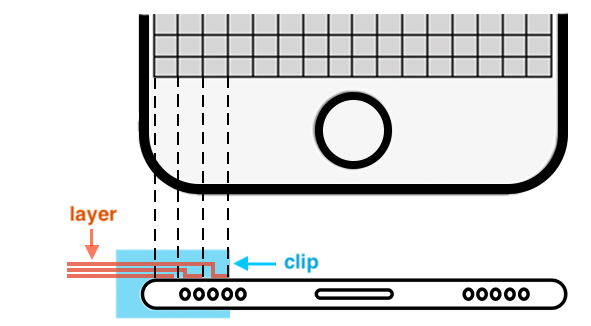
\includegraphics[width=0.25\columnwidth]{figures/3d_layout.png}
  \setlength{\belowcaptionskip}{-6pt}
  \caption{Possible design for more sensing nodes. }
  \label{fig:3d layout}
\end{figure}

\section{Conclusion}
\textit{FlexTouch} enables large-scale, passive, and low-cost interaction sensing interfaces by extending the capacitive sensing capability of touchscreens into the ambient environment. It can support a variety of large-scale interaction applications by attaching customized conductive strips to the edge of the touchscreen. We demonstrated that our technique allows for easy fabrication of touch interfaces via a variety of commercially available conductive materials and fabrication approaches. Through a series of evaluation studies, we showed that \textit{FlexTouch} supports long-range touch interaction sensing for up to 4 meters as well as everyday object presence detection for up to 2 meters. Then we demonstrated the versatility and feasibility of \textit{FlexTouch} by implementing and evaluating applications in the domain of body posture recognition, activity detection, object presence detection, and enhanced fitness tracking experiences.



%%% 其它部分
\backmatter

%% 本科生要这几个索引,研究生不要。选择性留下。
% 插图索引
% \listoffigures
% 表格索引
% \listoftables
% 公式索引
% \listofequations


%% 参考文献
% 注意:至少需要引用一篇参考文献,否则下面两行可能引起编译错误。
% 如果不需要参考文献,请将下面两行删除或注释掉。
\bibliographystyle{thuthesis-numeric}      % 顺序编码制
% \bibliographystyle{thuthesis-author-year}  % 著者-出版年制
% \bibliographystyle{thuthesis-bachelor}     % 本科生参考文献的著录格式
\bibliography{ref/refs}


%% 致谢
% 如果使用声明扫描页,将可选参数指定为扫描后的 PDF 文件名,例如:
% \begin{acknowledgement}[scan-statement.pdf]
\begin{acknowledgement}
    We would like to thank all our study participants for their time, effort, and patience. We would like to thank Maggie Chen for the demo video voiceover and Matt Andryc for his constructive comments. Our work is supported by the National Key Research and Development Plan of China under Grant No. 2016YFB1001402, the Natural Science Foundation of China under Grant No.: 61521002 and 61572276. Our work is also supported by the Beijing Key Lab of Networked Multimedia,  Undergraduate / Graduate Education Innovation Grants, Tsinghua University.
\end{acknowledgement}


%% 附录
\begin{appendix}
% \chapter{外文资料原文}
\label{cha:engorg}

\title{The title of the English paper}

\textbf{Abstract:} As one of the most widely used techniques in operations
research, \emph{ mathematical programming} is defined as a means of maximizing a
quantity known as \emph{bjective function}, subject to a set of constraints
represented by equations and inequalities. Some known subtopics of mathematical
programming are linear programming, nonlinear programming, multiobjective
programming, goal programming, dynamic programming, and multilevel
programming$^{[1]}$.

It is impossible to cover in a single chapter every concept of mathematical
programming. This chapter introduces only the basic concepts and techniques of
mathematical programming such that readers gain an understanding of them
throughout the book$^{[2,3]}$.


\section{Single-Objective Programming}
The general form of single-objective programming (SOP) is written
as follows,
\begin{equation*} % 如果附录中的公式不想让它出现在公式索引中,那就请
                             % 用 equation*
\left\{\begin{array}{l}
\max \,\,f(x)\\[0.1 cm]
\mbox{subject to:} \\ [0.1 cm]
\qquad g_j(x)\le 0,\quad j=1,2,\cdots,p
\end{array}\right.
\end{equation*}
which maximizes a real-valued function $f$ of
$x=(x_1,x_2,\cdots,x_n)$ subject to a set of constraints.

\newcommand\Real{\mathbf{R}}
\newtheorem{mpdef}{Definition}[chapter]
\begin{mpdef}
In SOP, we call $x$ a decision vector, and
$x_1,x_2,\cdots,x_n$ decision variables. The function
$f$ is called the objective function. The set
\begin{equation*}
S=\left\{x\in\Real^n\bigm|g_j(x)\le 0,\,j=1,2,\cdots,p\right\}
\end{equation*}
is called the feasible set. An element $x$ in $S$ is called a
feasible solution.
\end{mpdef}

\newtheorem{mpdefop}[mpdef]{Definition}
\begin{mpdefop}
A feasible solution $x^*$ is called the optimal
solution of SOP if and only if
\begin{equation}
f(x^*)\ge f(x)
\end{equation}
for any feasible solution $x$.
\end{mpdefop}

One of the outstanding contributions to mathematical programming was known as
the Kuhn-Tucker conditions\ref{eq:ktc}. In order to introduce them, let us give
some definitions. An inequality constraint $g_j(x)\le 0$ is said to be active at
a point $x^*$ if $g_j(x^*)=0$. A point $x^*$ satisfying $g_j(x^*)\le 0$ is said
to be regular if the gradient vectors $\nabla g_j(x)$ of all active constraints
are linearly independent.

Let $x^*$ be a regular point of the constraints of SOP and assume that all the
functions $f(x)$ and $g_j(x),j=1,2,\cdots,p$ are differentiable. If $x^*$ is a
local optimal solution, then there exist Lagrange multipliers
$\lambda_j,j=1,2,\cdots,p$ such that the following Kuhn-Tucker conditions hold,
\begin{equation}
\label{eq:ktc}
\left\{\begin{array}{l}
    \nabla f(x^*)-\sum\limits_{j=1}^p\lambda_j\nabla g_j(x^*)=0\\[0.3cm]
    \lambda_jg_j(x^*)=0,\quad j=1,2,\cdots,p\\[0.2cm]
    \lambda_j\ge 0,\quad j=1,2,\cdots,p.
\end{array}\right.
\end{equation}
If all the functions $f(x)$ and $g_j(x),j=1,2,\cdots,p$ are convex and
differentiable, and the point $x^*$ satisfies the Kuhn-Tucker conditions
(\ref{eq:ktc}), then it has been proved that the point $x^*$ is a global optimal
solution of SOP.

\subsection{Linear Programming}
\label{sec:lp}

If the functions $f(x),g_j(x),j=1,2,\cdots,p$ are all linear, then SOP is called
a {\em linear programming}.

The feasible set of linear is always convex. A point $x$ is called an extreme
point of convex set $S$ if $x\in S$ and $x$ cannot be expressed as a convex
combination of two points in $S$. It has been shown that the optimal solution to
linear programming corresponds to an extreme point of its feasible set provided
that the feasible set $S$ is bounded. This fact is the basis of the {\em simplex
  algorithm} which was developed by Dantzig as a very efficient method for
solving linear programming.
\begin{table}[ht]
\centering
  \centering
  \caption*{Table~1\hskip1em This is an example for manually numbered table, which
    would not appear in the list of tables}
  \label{tab:badtabular2}
  \begin{tabular}[c]{|m{1.5cm}|c|c|c|c|c|c|}\hline
    \multicolumn{2}{|c|}{Network Topology} & \# of nodes &
    \multicolumn{3}{c|}{\# of clients} & Server \\\hline
    GT-ITM & Waxman Transit-Stub & 600 &
    \multirow{2}{2em}{2\%}&
    \multirow{2}{2em}{10\%}&
    \multirow{2}{2em}{50\%}&
    \multirow{2}{1.2in}{Max. Connectivity}\\\cline{1-3}
    \multicolumn{2}{|c|}{Inet-2.1} & 6000 & & & &\\\hline
    \multirow{2}{1.5cm}{Xue} & Rui  & Ni &\multicolumn{4}{c|}{\multirow{2}*{\thuthesis}}\\\cline{2-3}
    & \multicolumn{2}{c|}{ABCDEF} &\multicolumn{4}{c|}{} \\\hline
\end{tabular}
\end{table}

Roughly speaking, the simplex algorithm examines only the extreme points of the
feasible set, rather than all feasible points. At first, the simplex algorithm
selects an extreme point as the initial point. The successive extreme point is
selected so as to improve the objective function value. The procedure is
repeated until no improvement in objective function value can be made. The last
extreme point is the optimal solution.

\subsection{Nonlinear Programming}

If at least one of the functions $f(x),g_j(x),j=1,2,\cdots,p$ is nonlinear, then
SOP is called a {\em nonlinear programming}.

A large number of classical optimization methods have been developed to treat
special-structural nonlinear programming based on the mathematical theory
concerned with analyzing the structure of problems.
\begin{figure}[h]
  \centering
  
\includegraphics{thu-lib-logo.pdf}
  \caption*{Figure~1\quad This is an example for manually numbered figure,
    which would not appear in the list of figures}
  \label{tab:badfigure2}
\end{figure}

Now we consider a nonlinear programming which is confronted solely with
maximizing a real-valued function with domain $\Real^n$.  Whether derivatives are
available or not, the usual strategy is first to select a point in $\Real^n$ which
is thought to be the most likely place where the maximum exists. If there is no
information available on which to base such a selection, a point is chosen at
random. From this first point an attempt is made to construct a sequence of
points, each of which yields an improved objective function value over its
predecessor. The next point to be added to the sequence is chosen by analyzing
the behavior of the function at the previous points. This construction continues
until some termination criterion is met. Methods based upon this strategy are
called {\em ascent methods}, which can be classified as {\em direct methods},
{\em gradient methods}, and {\em Hessian methods} according to the information
about the behavior of objective function $f$. Direct methods require only that
the function can be evaluated at each point. Gradient methods require the
evaluation of first derivatives of $f$. Hessian methods require the evaluation
of second derivatives. In fact, there is no superior method for all
problems. The efficiency of a method is very much dependent upon the objective
function.

\subsection{Integer Programming}

{\em Integer programming} is a special mathematical programming in which all of
the variables are assumed to be only integer values. When there are not only
integer variables but also conventional continuous variables, we call it {\em
  mixed integer programming}. If all the variables are assumed either 0 or 1,
then the problem is termed a {\em zero-one programming}. Although integer
programming can be solved by an {\em exhaustive enumeration} theoretically, it
is impractical to solve realistically sized integer programming problems. The
most successful algorithm so far found to solve integer programming is called
the {\em branch-and-bound enumeration} developed by Balas (1965) and Dakin
(1965). The other technique to integer programming is the {\em cutting plane
  method} developed by Gomory (1959).

\hfill\textit{Uncertain Programming\/}\quad(\textsl{BaoDing Liu, 2006.2})

\section*{References}
\noindent{\itshape NOTE: These references are only for demonstration. They are
  not real citations in the original text.}

\begin{translationbib}
\item Donald E. Knuth. The \TeX book. Addison-Wesley, 1984. ISBN: 0-201-13448-9
\item Paul W. Abrahams, Karl Berry and Kathryn A. Hargreaves. \TeX\ for the
  Impatient. Addison-Wesley, 1990. ISBN: 0-201-51375-7
\item David Salomon. The advanced \TeX book.  New York : Springer, 1995. ISBN:0-387-94556-3
\end{translationbib}

\chapter{外文资料的调研阅读报告或书面翻译}

\title{英文资料的中文标题}

{\heiti 摘要:} 本章为外文资料翻译内容。如果有摘要可以直接写上来,这部分好像没有
明确的规定。

\section{单目标规划}
北冥有鱼,其名为鲲。鲲之大,不知其几千里也。化而为鸟,其名为鹏。鹏之背,不知其几
千里也。怒而飞,其翼若垂天之云。是鸟也,海运则将徙于南冥。南冥者,天池也。
\begin{equation}\tag*{(123)}
 p(y|\mathbf{x}) = \frac{p(\mathbf{x},y)}{p(\mathbf{x})}=
\frac{p(\mathbf{x}|y)p(y)}{p(\mathbf{x})}
\end{equation}

吾生也有涯,而知也无涯。以有涯随无涯,殆已!已而为知者,殆而已矣!为善无近名,为
恶无近刑,缘督以为经,可以保身,可以全生,可以养亲,可以尽年。

\subsection{线性规划}
庖丁为文惠君解牛,手之所触,肩之所倚,足之所履,膝之所倚,砉然响然,奏刀騞然,莫
不中音,合于桑林之舞,乃中经首之会。
\begin{table}[ht]
\centering
  \centering
  \caption*{表~1\hskip1em 这是手动编号但不出现在索引中的一个表格例子}
  \label{tab:badtabular3}
  \begin{tabular}[c]{|m{1.5cm}|c|c|c|c|c|c|}\hline
    \multicolumn{2}{|c|}{Network Topology} & \# of nodes &
    \multicolumn{3}{c|}{\# of clients} & Server \\\hline
    GT-ITM & Waxman Transit-Stub & 600 &
    \multirow{2}{2em}{2\%}&
    \multirow{2}{2em}{10\%}&
    \multirow{2}{2em}{50\%}&
    \multirow{2}{1.2in}{Max. Connectivity}\\\cline{1-3}
    \multicolumn{2}{|c|}{Inet-2.1} & 6000 & & & &\\\hline
    \multirow{2}{1.5cm}{Xue} & Rui  & Ni &\multicolumn{4}{c|}{\multirow{2}*{\thuthesis}}\\\cline{2-3}
    & \multicolumn{2}{c|}{ABCDEF} &\multicolumn{4}{c|}{} \\\hline
\end{tabular}
\end{table}

文惠君曰:“嘻,善哉!技盖至此乎?”庖丁释刀对曰:“臣之所好者道也,进乎技矣。始臣之
解牛之时,所见无非全牛者;三年之后,未尝见全牛也;方今之时,臣以神遇而不以目视,
官知止而神欲行。依乎天理,批大郤,导大窾,因其固然。技经肯綮之未尝,而况大坬乎!
良庖岁更刀,割也;族庖月更刀,折也;今臣之刀十九年矣,所解数千牛矣,而刀刃若新发
于硎。彼节者有间而刀刃者无厚,以无厚入有间,恢恢乎其于游刃必有余地矣。是以十九年
而刀刃若新发于硎。虽然,每至于族,吾见其难为,怵然为戒,视为止,行为迟,动刀甚微,
謋然已解,如土委地。提刀而立,为之而四顾,为之踌躇满志,善刀而藏之。”

文惠君曰:“善哉!吾闻庖丁之言,得养生焉。”


\subsection{非线性规划}
孔子与柳下季为友,柳下季之弟名曰盗跖。盗跖从卒九千人,横行天下,侵暴诸侯。穴室枢
户,驱人牛马,取人妇女。贪得忘亲,不顾父母兄弟,不祭先祖。所过之邑,大国守城,小
国入保,万民苦之。孔子谓柳下季曰:“夫为人父者,必能诏其子;为人兄者,必能教其弟。
若父不能诏其子,兄不能教其弟,则无贵父子兄弟之亲矣。今先生,世之才士也,弟为盗
跖,为天下害,而弗能教也,丘窃为先生羞之。丘请为先生往说之。”
\begin{figure}[h]
  \centering
  
\includegraphics{thu-whole-logo.pdf}
  \caption*{图~1\hskip1em 这是手动编号但不出现索引中的图片的例子}
  \label{tab:badfigure3}
\end{figure}

柳下季曰:“先生言为人父者必能诏其子,为人兄者必能教其弟,若子不听父之诏,弟不受
兄之教,虽今先生之辩,将奈之何哉?且跖之为人也,心如涌泉,意如飘风,强足以距敌,
辩足以饰非。顺其心则喜,逆其心则怒,易辱人以言。先生必无往。”

孔子不听,颜回为驭,子贡为右,往见盗跖。

\subsection{整数规划}
盗跖乃方休卒徒大山之阳,脍人肝而餔之。孔子下车而前,见谒者曰:“鲁人孔丘,闻将军
高义,敬再拜谒者。”谒者入通。盗跖闻之大怒,目如明星,发上指冠,曰:“此夫鲁国之
巧伪人孔丘非邪?为我告之:尔作言造语,妄称文、武,冠枝木之冠,带死牛之胁,多辞缪
说,不耕而食,不织而衣,摇唇鼓舌,擅生是非,以迷天下之主,使天下学士不反其本,妄
作孝弟,而侥幸于封侯富贵者也。子之罪大极重,疾走归!不然,我将以子肝益昼餔之膳。”


\chapter{其它附录}
前面两个附录主要是给本科生做例子。其它附录的内容可以放到这里,当然如果你愿意,可
以把这部分也放到独立的文件中,然后将其 \cs{input} 到主文件中。

\end{appendix}

%% 个人简历
\begin{resume}

  \resumeitem{Education}

Sep 2013–Jul 2017, Bachelor of Science in Engineering in Control Science and Technology, Tsinghua University.

Sep 2017-Jul 2019, Master of Science in Technology Innovation, University of Washington.

Sep 2017-Jul 2019, Master of Science in Engineering in Data Science and Information Technology, Tsinghua University.

\resumeitem{Awards}
Jun 2018, Second Prize of the National University Blockchain Competition in North China.

Oct 2017, Third Prize of National College Students Innovation and Entrepreneurship Competition.


%   \researchitem{Awards} % 发表的和录用的合在一起

%   % 1. 已经刊载的学术论文(本人是第一作者,或者导师为第一作者本人是第二作者)
%   \begin{publications}
%     \item 杨轶, 张宁欣, 任天令, 等. 硅基铁电微声学器件中薄膜残余应力的研究. 中国机
%       械工程, 2005, 16(14):1289-1291. (EI 收录, 检索号:0534931 2907.)
%   \end{publications}

%   % 2. 尚未刊载,但已经接到正式录用函的学术论文(本人为第一作者,或者
%   %    导师为第一作者本人是第二作者)。
%   \begin{publications}[before=\publicationskip,after=\publicationskip]
%     \item Yang Y, Ren T L, Zhu Y P, et al. PMUTs for handwriting recognition. In
%       press. (已被 Integrated Ferroelectrics 录用. SCI 源刊.)
%   \end{publications}

%   % 3. 其他学术论文。可列出除上述两种情况以外的其他学术论文,但必须是
%   %    已经刊载或者收到正式录用函的论文。
%   \begin{publications}
%     \item Wu X M, Yang Y, Cai J, et al. Measurements of ferroelectric MEMS
%       microphones. Integrated Ferroelectrics, 2005, 69:417-429. (SCI 收录, 检索号
%       :896KM)
%     \item 贾泽, 杨轶, 陈兢, 等. 用于压电和电容微麦克风的体硅腐蚀相关研究. 压电与声
%       光, 2006, 28(1):117-119. (EI 收录, 检索号:06129773469)
%     \item 伍晓明, 杨轶, 张宁欣, 等. 基于MEMS技术的集成铁电硅微麦克风. 中国集成电路,
%       2003, 53:59-61.
%   \end{publications}

%   \researchitem{研究成果} % 有就写,没有就删除
%   \begin{achievements}
%     \item 任天令, 杨轶, 朱一平, 等. 硅基铁电微声学传感器畴极化区域控制和电极连接的
%       方法: 中国, CN1602118A. (中国专利公开号)
%   \end{achievements}

\end{resume}


%% 本科生进行格式审查是需要下面这个表格,答辩可能不需要。选择性留下。
% 综合论文训练记录表
% 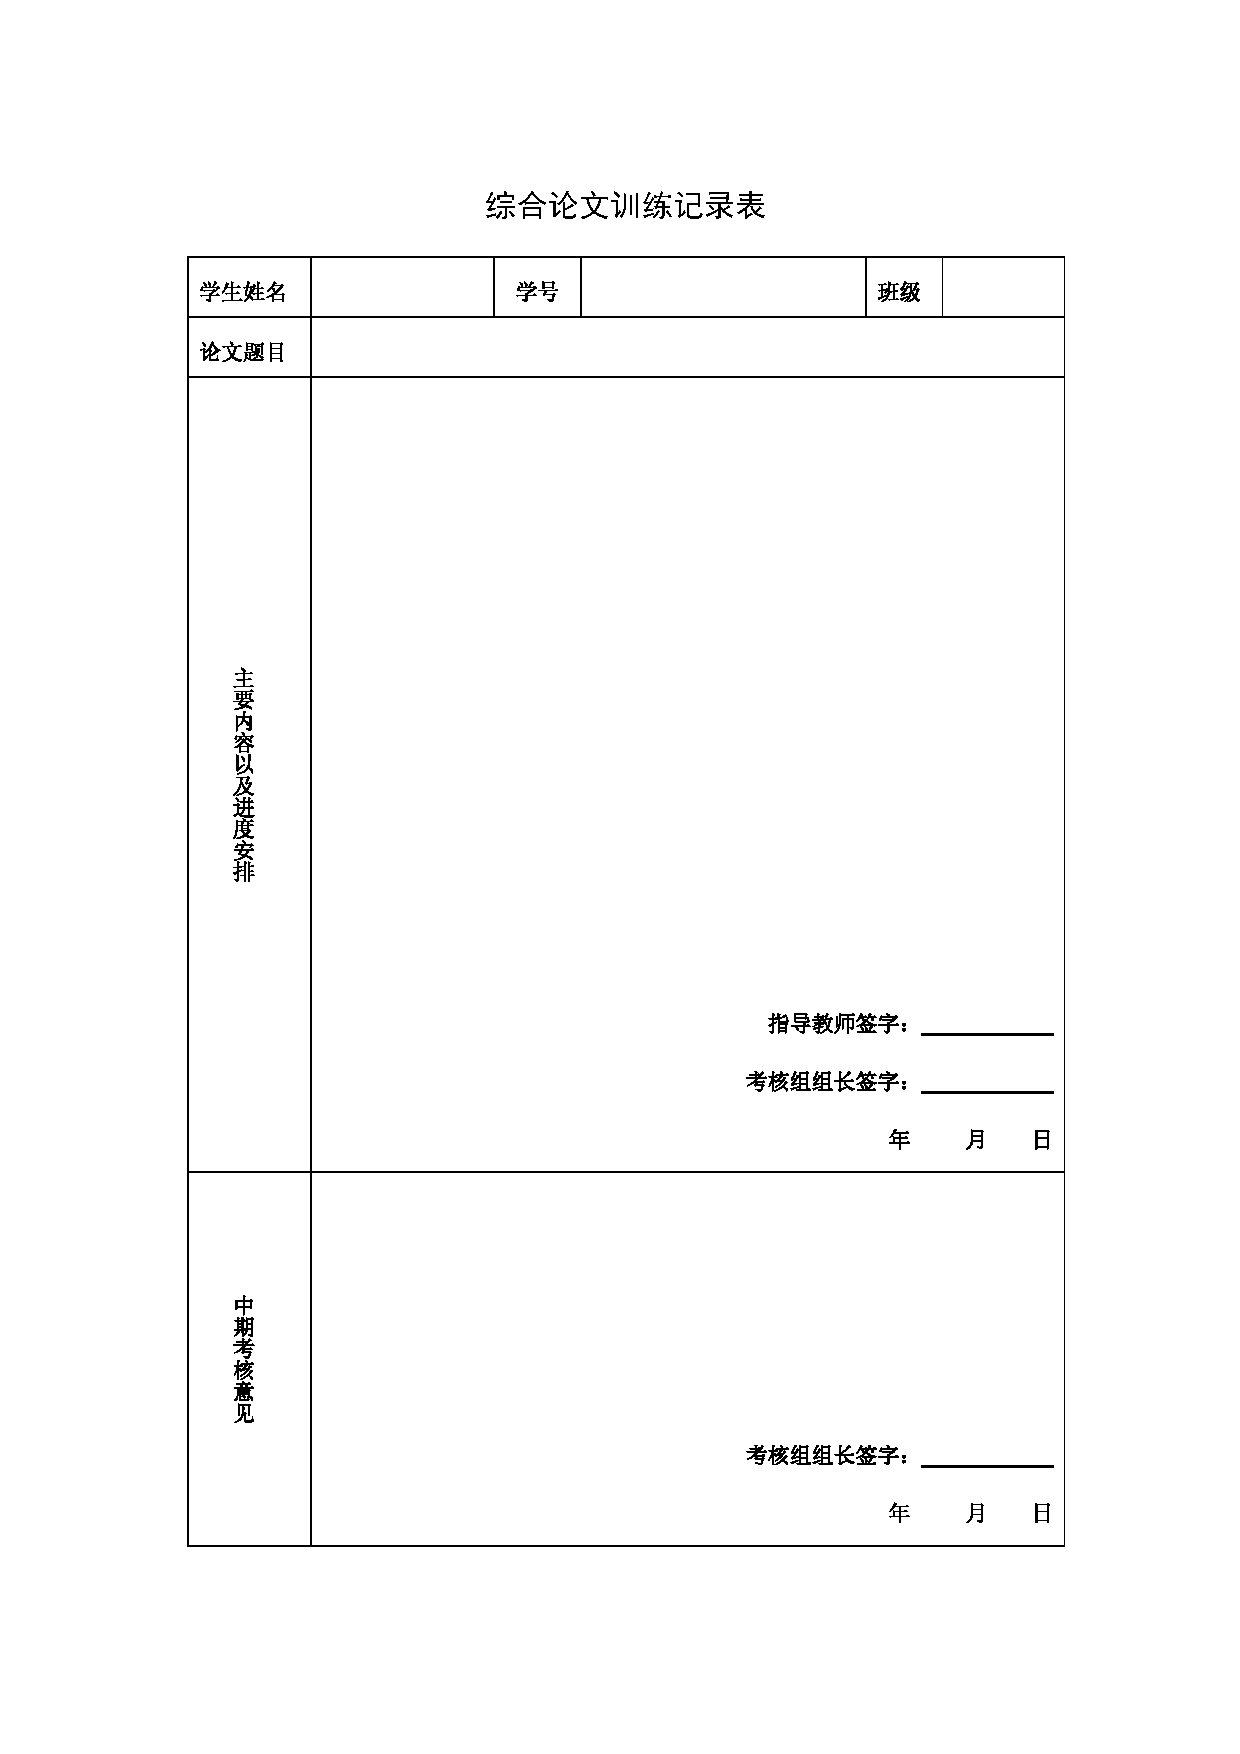
\includepdf[pages=-]{scan-record.pdf}
\end{document}
